% Options for packages loaded elsewhere
\PassOptionsToPackage{unicode}{hyperref}
\PassOptionsToPackage{hyphens}{url}
\PassOptionsToPackage{dvipsnames,svgnames,x11names}{xcolor}
%
\documentclass[
  12pt,
  letterpaper,
  DIV=11,
  numbers=noendperiod]{scrreprt}

\usepackage{amsmath,amssymb}
\usepackage{iftex}
\ifPDFTeX
  \usepackage[T1]{fontenc}
  \usepackage[utf8]{inputenc}
  \usepackage{textcomp} % provide euro and other symbols
\else % if luatex or xetex
  \usepackage{unicode-math}
  \defaultfontfeatures{Scale=MatchLowercase}
  \defaultfontfeatures[\rmfamily]{Ligatures=TeX,Scale=1}
\fi
\usepackage{lmodern}
\ifPDFTeX\else  
    % xetex/luatex font selection
\fi
% Use upquote if available, for straight quotes in verbatim environments
\IfFileExists{upquote.sty}{\usepackage{upquote}}{}
\IfFileExists{microtype.sty}{% use microtype if available
  \usepackage[]{microtype}
  \UseMicrotypeSet[protrusion]{basicmath} % disable protrusion for tt fonts
}{}
\makeatletter
\@ifundefined{KOMAClassName}{% if non-KOMA class
  \IfFileExists{parskip.sty}{%
    \usepackage{parskip}
  }{% else
    \setlength{\parindent}{0pt}
    \setlength{\parskip}{6pt plus 2pt minus 1pt}}
}{% if KOMA class
  \KOMAoptions{parskip=half}}
\makeatother
\usepackage{xcolor}
\usepackage[margin=2.5cm]{geometry}
\setlength{\emergencystretch}{3em} % prevent overfull lines
\setcounter{secnumdepth}{5}
% Make \paragraph and \subparagraph free-standing
\makeatletter
\ifx\paragraph\undefined\else
  \let\oldparagraph\paragraph
  \renewcommand{\paragraph}{
    \@ifstar
      \xxxParagraphStar
      \xxxParagraphNoStar
  }
  \newcommand{\xxxParagraphStar}[1]{\oldparagraph*{#1}\mbox{}}
  \newcommand{\xxxParagraphNoStar}[1]{\oldparagraph{#1}\mbox{}}
\fi
\ifx\subparagraph\undefined\else
  \let\oldsubparagraph\subparagraph
  \renewcommand{\subparagraph}{
    \@ifstar
      \xxxSubParagraphStar
      \xxxSubParagraphNoStar
  }
  \newcommand{\xxxSubParagraphStar}[1]{\oldsubparagraph*{#1}\mbox{}}
  \newcommand{\xxxSubParagraphNoStar}[1]{\oldsubparagraph{#1}\mbox{}}
\fi
\makeatother


\providecommand{\tightlist}{%
  \setlength{\itemsep}{0pt}\setlength{\parskip}{0pt}}\usepackage{longtable,booktabs,array}
\usepackage{calc} % for calculating minipage widths
% Correct order of tables after \paragraph or \subparagraph
\usepackage{etoolbox}
\makeatletter
\patchcmd\longtable{\par}{\if@noskipsec\mbox{}\fi\par}{}{}
\makeatother
% Allow footnotes in longtable head/foot
\IfFileExists{footnotehyper.sty}{\usepackage{footnotehyper}}{\usepackage{footnote}}
\makesavenoteenv{longtable}
\usepackage{graphicx}
\makeatletter
\def\maxwidth{\ifdim\Gin@nat@width>\linewidth\linewidth\else\Gin@nat@width\fi}
\def\maxheight{\ifdim\Gin@nat@height>\textheight\textheight\else\Gin@nat@height\fi}
\makeatother
% Scale images if necessary, so that they will not overflow the page
% margins by default, and it is still possible to overwrite the defaults
% using explicit options in \includegraphics[width, height, ...]{}
\setkeys{Gin}{width=\maxwidth,height=\maxheight,keepaspectratio}
% Set default figure placement to htbp
\makeatletter
\def\fps@figure{htbp}
\makeatother
% definitions for citeproc citations
\NewDocumentCommand\citeproctext{}{}
\NewDocumentCommand\citeproc{mm}{%
  \begingroup\def\citeproctext{#2}\cite{#1}\endgroup}
\makeatletter
 % allow citations to break across lines
 \let\@cite@ofmt\@firstofone
 % avoid brackets around text for \cite:
 \def\@biblabel#1{}
 \def\@cite#1#2{{#1\if@tempswa , #2\fi}}
\makeatother
\newlength{\cslhangindent}
\setlength{\cslhangindent}{1.5em}
\newlength{\csllabelwidth}
\setlength{\csllabelwidth}{3em}
\newenvironment{CSLReferences}[2] % #1 hanging-indent, #2 entry-spacing
 {\begin{list}{}{%
  \setlength{\itemindent}{0pt}
  \setlength{\leftmargin}{0pt}
  \setlength{\parsep}{0pt}
  % turn on hanging indent if param 1 is 1
  \ifodd #1
   \setlength{\leftmargin}{\cslhangindent}
   \setlength{\itemindent}{-1\cslhangindent}
  \fi
  % set entry spacing
  \setlength{\itemsep}{#2\baselineskip}}}
 {\end{list}}
\usepackage{calc}
\newcommand{\CSLBlock}[1]{\hfill\break\parbox[t]{\linewidth}{\strut\ignorespaces#1\strut}}
\newcommand{\CSLLeftMargin}[1]{\parbox[t]{\csllabelwidth}{\strut#1\strut}}
\newcommand{\CSLRightInline}[1]{\parbox[t]{\linewidth - \csllabelwidth}{\strut#1\strut}}
\newcommand{\CSLIndent}[1]{\hspace{\cslhangindent}#1}

\usepackage{booktabs}
\usepackage{longtable}
\usepackage{array}
\usepackage{multirow}
\usepackage{wrapfig}
\usepackage{float}
\usepackage{colortbl}
\usepackage{pdflscape}
\usepackage{tabu}
\usepackage{threeparttable}
\usepackage{threeparttablex}
\usepackage[normalem]{ulem}
\usepackage{makecell}
\usepackage{xcolor}
\KOMAoption{captions}{tableheading}
\makeatletter
\@ifpackageloaded{bookmark}{}{\usepackage{bookmark}}
\makeatother
\makeatletter
\@ifpackageloaded{caption}{}{\usepackage{caption}}
\AtBeginDocument{%
\ifdefined\contentsname
  \renewcommand*\contentsname{Índice}
\else
  \newcommand\contentsname{Índice}
\fi
\ifdefined\listfigurename
  \renewcommand*\listfigurename{Lista de Figuras}
\else
  \newcommand\listfigurename{Lista de Figuras}
\fi
\ifdefined\listtablename
  \renewcommand*\listtablename{Lista de Tabelas}
\else
  \newcommand\listtablename{Lista de Tabelas}
\fi
\ifdefined\figurename
  \renewcommand*\figurename{Figura}
\else
  \newcommand\figurename{Figura}
\fi
\ifdefined\tablename
  \renewcommand*\tablename{Tabela}
\else
  \newcommand\tablename{Tabela}
\fi
}
\@ifpackageloaded{float}{}{\usepackage{float}}
\floatstyle{ruled}
\@ifundefined{c@chapter}{\newfloat{codelisting}{h}{lop}}{\newfloat{codelisting}{h}{lop}[chapter]}
\floatname{codelisting}{Listagem}
\newcommand*\listoflistings{\listof{codelisting}{Lista de Listagens}}
\makeatother
\makeatletter
\makeatother
\makeatletter
\@ifpackageloaded{caption}{}{\usepackage{caption}}
\@ifpackageloaded{subcaption}{}{\usepackage{subcaption}}
\makeatother

\ifLuaTeX
\usepackage[bidi=basic]{babel}
\else
\usepackage[bidi=default]{babel}
\fi
\babelprovide[main,import]{portuguese}
% get rid of language-specific shorthands (see #6817):
\let\LanguageShortHands\languageshorthands
\def\languageshorthands#1{}
\ifLuaTeX
  \usepackage{selnolig}  % disable illegal ligatures
\fi
\usepackage{bookmark}

\IfFileExists{xurl.sty}{\usepackage{xurl}}{} % add URL line breaks if available
\urlstyle{same} % disable monospaced font for URLs
\hypersetup{
  pdftitle={Análise de Sobrevivência},
  pdfauthor={Breno Cauã Rodrigues da Silva},
  pdflang={pt},
  colorlinks=true,
  linkcolor={blue},
  filecolor={Maroon},
  citecolor={Blue},
  urlcolor={Blue},
  pdfcreator={LaTeX via pandoc}}


\title{Análise de Sobrevivência}
\usepackage{etoolbox}
\makeatletter
\providecommand{\subtitle}[1]{% add subtitle to \maketitle
  \apptocmd{\@title}{\par {\large #1 \par}}{}{}
}
\makeatother
\subtitle{Iniciação Ciêntifica - PIBIC 2024/2025 (UFPA)}
\author{\textbf{Breno Cauã Rodrigues da Silva}}
\date{2024-01-25}

\begin{document}
\maketitle

\renewcommand*\contentsname{Índice}
{
\hypersetup{linkcolor=}
\setcounter{tocdepth}{2}
\tableofcontents
}

\bookmarksetup{startatroot}

\chapter*{Prefácio}\label{prefuxe1cio}
\addcontentsline{toc}{chapter}{Prefácio}

\markboth{Prefácio}{Prefácio}

Este é um projeto desenvolvido\ldots{}

\bookmarksetup{startatroot}

\chapter{Conceitos Básicos e
Exemplos}\label{conceitos-buxe1sicos-e-exemplos}

\section{Introdução}\label{introduuxe7uxe3o}

O objetivo deste capítulo inicial é apresentar alguns \emph{conceitos} e
\emph{fundamentos} de uma das áreas da Estatística e Análise de Dados
que mais se desenvolveram nas últimas duas décadas do século XX. Esse
avanço foi impulsionado pela evolução das técnicas estatísticas aliada
ao progresso computacional.

Na Análise de Sobrevivência, a variável resposta é, em geral, o
\emph{tempo até a ocorrência de um evento de interesse}.
Especificamente, essa área se concentra em modelar e compreender o tempo
necessário para que um evento significativo ocorra, sendo este
denominado \textbf{tempo de falha}. Como exemplo, Colosimo e Giolo
(2006) mencionam casos como o tempo até a morte de um paciente, até a
cura de uma doença ou até a recidiva de uma condição clínica.

Uma questão frequentemente levantada é: por que não utilizar outras
técnicas estatísticas? Métodos tradicionais não são adequados para dados
de sobrevivência devido a uma característica única: a \textbf{censura}.
Esse conceito refere-se à observação parcial do tempo de falha, como
ocorre quando o acompanhamento de um paciente é interrompido antes do
evento de interesse. A censura, sendo um elemento essencial da Análise
de Sobrevivência, caracteriza situações em que o tempo de falha real é
desconhecido, sabendo-se apenas que ele excede determinado ponto.

\section{Tempo de Falha}\label{tempo-de-falha}

Na Análise de Sobrevivência, é fundamental estabelecer alguns pontos
iniciais para o estudo. O primeiro deles é o \textbf{tempo inicial do
estudo}, que deve ser claramente definido para garantir que os
indivíduos sejam comparáveis no ponto de partida, diferenciando-se
apenas pelas covariáveis medidas. Existem diversas maneiras de definir o
tempo inicial, sendo o mais comum o \textbf{tempo cronológico}. Contudo,
em áreas como Engenharia, outras métricas, como número de ciclos ou
quilometragem, também podem ser utilizadas. Colosimo e Giolo (2006)
apresentam exemplos práticos, como medidas de carga para equipamentos.

Outro aspecto essencial é a \textbf{definição do evento de interesse},
frequentemente associado a falhas ou situações indesejáveis. Para
garantir resultados consistentes, a definição do evento deve ser clara e
objetiva. Um exemplo elucidativo é fornecido por Colosimo e Giolo
(2006):

\begin{quote}
\emph{``Em algumas situações, a definição de falha já é clara, como
morte ou recidiva, mas em outras pode assumir termos ambíguos. Por
exemplo, fabricantes de produtos alimentícios desejam saber o tempo de
vida de seus produtos expostos em balcões frigoríficos de supermercados.
O tempo de falha vai do momento de exposição (chegada ao supermercado)
até o produto se tornar `inapropriado para consumo'. Esse evento deve
ser claramente definido antes do início do estudo. Por exemplo, o
produto é considerado inapropriado para consumo quando atinge uma
concentração específica de microrganismos por} \(mm^{2}\) \emph{de
área.''}
\end{quote}

\section{Censura}\label{censura}

Estudos clínicos que tratam a resposta como uma variável temporal
geralmente são prospectivos e de longa duração. No entanto, mesmo sendo
extensos, esses estudos frequentemente se encerram antes que todos os
indivíduos passem pelo evento de interesse.

Uma característica comum nesses estudos é a \textbf{censura}, que
corresponde a observações incompletas ou parciais. Apesar disso, tais
observações fornecem informações valiosas para a análise. Colosimo e
Giolo (2006) destacam a relevância de incluir dados censurados na
análise:

\begin{quote}
\emph{``Ressalta-se que, mesmo censurados, todos os resultados
provenientes de um estudo de sobrevivência devem ser incluídos na
análise estatística. Duas razões justificam esse procedimento: (i) mesmo
sendo incompletas, as observações censuradas fornecem informações sobre
o tempo de vida dos pacientes; (ii) a exclusão das censuras no cálculo
das estatísticas pode levar a conclusões enviesadas.''}
\end{quote}

Existem três tipos principais de censura:

\begin{itemize}
\tightlist
\item
  \textbf{Censura Tipo I:} O estudo é encerrado após um período de tempo
  previamente definido.
\item
  \textbf{Censura Tipo II:} O estudo termina quando um número específico
  de indivíduos passa pelo evento de interesse.
\item
  \textbf{Censura Aleatória:} Ocorre quando um indivíduo é retirado do
  estudo antes do evento de interesse.
\end{itemize}

A censura mais comum é a \textbf{censura à direita}, em que o evento
ocorre após o tempo registrado. Entretanto, outros tipos de censura,
como \textbf{à esquerda} e \textbf{intervalar}, também são possíveis.

Censura à esquerda ocorre quando o evento já aconteceu antes do início
da observação. Um exemplo é um estudo sobre a idade em que crianças
aprendem a ler:

\begin{quote}
\emph{``Quando os pesquisadores começaram a pesquisa, algumas crianças
já sabiam ler e não se lembravam com que idade isso ocorreu,
caracterizando observações censuradas à esquerda.''}
\end{quote}

No mesmo estudo, observa-se censura à direita para crianças que ainda
não sabiam ler no momento da coleta de dados. Nesse caso, os tempos de
vida são classificados como \textbf{duplamente censurados} (Turnbull
1974).

A censura intervalar ocorre em estudos com visitas periódicas espaçadas,
onde só se sabe que o evento ocorreu dentro de um intervalo de tempo.
Quando o tempo de falha \(T\) é impreciso, considera-se que ele pertence
a um intervalo \(T \in (L, U]\), conhecido como \textbf{sobrevivência
intervalar}. Casos especiais incluem tempos de falha exatos, em que
\(L = U\), sendo \(U = 0\) para censura à direita e \(L = 0\) para
censura à esquerda (Lindsey e Ryan 1998). Destaca-se a seguinte
observação de Colosimo e Giolo (2006):

\begin{quote}
\emph{``A presença de censura traz desafios para a análise estatística.
A censura do Tipo II é, em princípio, mais tratável que os outros tipos,
mas para situações simples, que raramente ocorrem em estudos clínicos
(Lawless 1982). Na prática, utiliza-se resultados assintóticos para a
análise dos dados de sobrevivência.''}
\end{quote}

\section{Dados Truncados}\label{dados-truncados}

O truncamento é uma característica de alguns estudos de sobrevivência
que, muitas vezes, é confundida com a censura. Ele ocorre quando certos
indivíduos são excluídos do estudo devido a uma condição específica.
Nesse caso, os pacientes só são incluídos no acompanhamento após
passarem por um determinado evento, em vez de serem acompanhados desde o
início do processo.

\section{Representação dos Dados de Sobrevivência}\label{sec-ReprDados}

Considere uma amostra aleatória de tamanho \(n\). O \(i\)-ésimo
indivíduo no estudo é geralmente representado pelo par
\((t_{i}, \delta_{i})\), onde \(t_{i}\) é o tempo de falha ou censura,
indicado pela variável binária \(\delta_{i}\), definida como:

\[
\delta_{i} = \begin{cases}
1, & \text{se } t_{i} \text{ é um tempo de falha} \\
0, & \text{se } t_{i} \text{ é um tempo de censura}.
\end{cases}
\]

Portanto, a variável resposta na análise de sobrevivência é representada
por duas colunas no conjunto de dados.

Se o estudo também incluir covariáveis, os dados são representados por
\((t_{i}, \delta_{i}, \mathbf{x}i)\). Caso a censura seja intervalar, a
representação é \((l{i}, u_{i}, \delta_{i}, \mathbf{x}_i)\).

Para exemplos de dados de sobrevivência, veja a Seção 1.5 do livro de
Colosimo e Giolo (2006).

\section{Especificando o Tempo de
Sobrevivência}\label{especificando-o-tempo-de-sobrevivuxeancia}

Seja \(T\) uma variável aleatória (v.a.), na maioria dos casos contínua,
que representa o tempo de falha. Assim, o suporte de \(T\) é definido
nos reais positivos \(\mathbb{R}^{+}\). Tal variável é geralmente
representada pela sua \emph{função risco} ou pela \emph{função de taxa
de falha} (ou taxa de risco). Tais funções, e outras relacionadas, são
usadas ao longo do processo de análise de dados de sobrevivência. A
seguir, algumas dessas funções e as relações entre elas serão definidas.

\subsection{Função de
Sobrevivência}\label{funuxe7uxe3o-de-sobrevivuxeancia}

Esta é uma das principais funções probabilísticas usadas em análise de
sobrevivência. A função sobrevivência é definida como a probabilidade de
uma observação não falhar até certo ponto \(t\), ou seja a probabilidade
de uma observação sobreviver ao tempo \(t\). Em probabilidade, isso pode
ser escrito como:

\begin{equation}\phantomsection\label{eq-fSobrevida}{
S(t) = P(T > t),
}\end{equation}

uma conclusão a qual podemos chegar, é que a probabilidade de uma
observação não sobreviver até o tempo \(t\), é a acumulada até o ponto
\(t\), logo,

\begin{equation}\phantomsection\label{eq-complfSobrevida}{
F(t) = 1 - S(t).
}\end{equation}

\subsection{Função de Taxa de Falha ou de
Risco}\label{funuxe7uxe3o-de-taxa-de-falha-ou-de-risco}

A probabilidade da falha ocorrer em um intervalo de tempo
\([t_{1}, t_{2})\) pode ser expressa em termos da função de
sobrevivência como: \[S(t_{1}) - S(t_{2}).\]

A taxa de falha no intervalo \([t_{1}, t_{2})\) é definida como a
probabilidade de que a falha ocorra neste intervalo, dado que não
ocorreu antes de \(t_{1}\), dividida pelo comprimento do intervalo.
Assim, a taxa de falha no intervalo \([t_{1}, t_{2})\) é expressa por
\[\dfrac{S(t_{1}) - S(t_{2})}{(t_{2} - t_{1})S(t_{1})}.\]

De forma geral, redefinindo o intervalo como \([t, t + \Delta t)\) a
expressão assume a seguinte forma:

\[
\lambda(t) = \dfrac{S(t) - S(t + \Delta_{t})}{\Delta t \text{ } S(t)}
\]

Assumindo \(\Delta t\) bem pequeno, \(\lambda(t)\) representa a taxa de
falha instantânea no tempo \(t\) condicional à sobrevivência até o tempo
\(t\). Observe que as taxas de falha são números positivos, mas sem
limite superior. A função de taxa de falha \(\lambda(t)\) é bastante
útil para descrever a distribuição do tempo de vida de pacientes. Ela
descreve a forma em que a taxa instantânea de falha muda com o tempo. A
função de taxa de falha de \(T\) é, então, definida como:

\begin{equation}\phantomsection\label{eq-fTaxaFalha}{
\lambda(t) = \lim_{\Delta t \to 0} \dfrac{P(t \leq T \leq t + \Delta t | T \geq t)}{\Delta t}
}\end{equation}

A função de taxa de falha é mais informativa do que a função de
sobrevivência. Diferentes funções de sobrevivência podem ter formas
semelhantes, enquanto as respectivas funções de taxa de falha podem
diferir drasticamente. Desta forma, a modelagem da função de taxa de
falha é um importante método para dados de sobrevivência.

\subsection{Função de Taxa de Falha Acumulada}\label{sec-TaxaAcu}

Outra função útil em análise de dados de sobrevivência é a função taxa
de falha acumulada. Esta função, como o próprio nome sugere, fornece a
taxa de falha acumulada do indivíduo e é definida por:

\begin{equation}\phantomsection\label{eq-fTaxaFalhaAcumul}{
\Lambda(t) = \int_{0}^{t} \lambda(u) du.
}\end{equation}

A função de taxa de falha acumulada, \(\Lambda(t)\), não têm uma
interpretação direta, mas pode ser útil na avaliação da função de maior
interesse que é a função de taxa de falha, \(\lambda(t)\). Isto acontece
essencialmente na estimação não-paramétrica em que \(\Lambda(t)\)
apresenta um estimador com propriedades ótimas e \(\lambda(t)\) é
difícil de ser estimada.

\subsection{Tempo Médio e Vida Média
Residual}\label{tempo-muxe9dio-e-vida-muxe9dia-residual}

Outras duas quantidades de interesse em análise de sobrevivência são: o
tempo médio de via e a vida média residual. A primeira é obtida pela
área sob a função de sobrevivência. Isto é,

\begin{equation}\phantomsection\label{eq-TempMuxe9dio}{
t_{m} = \int_{0}^{\infty} S(t) dt.
}\end{equation}

Já a vida média residual é definida condicional a um certo tempo de vida
\(t\). Ou seja, para indivíduos com idade \(t\) está quantidade mede o
tempo médio restante de vida e é, então, a área sob a curva de
sobrevivência à direita do tempo \(t\) dividida por \(S(t)\). Isto é,

\begin{equation}\phantomsection\label{eq-TemVidaMediaResid}{
\text{vmr}(t) = \dfrac{\int_{0}^{\infty} (u - t) f(u) du}{S(t)} = \dfrac{\int_{0}^{\infty} S(u) du}{S(t)},
}\end{equation}

sendo \(f(\cdot)\) a função densidade de \(T\). Observe que
\(\text{vmr}(0) = t_{m}\).

\section{Relações entre as
Funções}\label{relauxe7uxf5es-entre-as-funuxe7uxf5es}

Para \(T\) uma variável aleatória contínua e não-negativa, tem-se, em
termos das funções definidas anteriormente, algumas relações matemáticas
importantes entre elas, a saber:

\[
\lambda(t) = \dfrac{f(t)}{S(t)} = - \dfrac{d}{dt} \left[ \log S(t) \right],
\]

\[
\Lambda(t) = \int_0^{t} \lambda(u) du = - \log S(t)
\]

e

\[
S(t) = \exp \left\{ - \Lambda(t) \right\} = \exp \left\{ - \int_0^{t} \lambda(u) du \right\}
\]

Tais relações mostram que o conhecimento de uma das funções, por exemplo
\(S(t)\), implica no conhecimento das demais, isto é, \(F(t)\),
\(f(t)\), \(\lambda(t)\) e \(\Lambda(t)\). Outras relações envolvendo
estas funções são as seguintes:

\[ 
S(t) = \dfrac{\text{vmr}(0)}{\text{vmr}(t)} \exp \left\{ - \int_{0}^{t} \dfrac{du}{\text{vmr}(u)} \right\}
\]

e

\[
\lambda(t) = \left( \dfrac{d \text{ } [\text{vmr}(t)]}{dt} + 1 \right) / \text{vmr}(t).
\]

\bookmarksetup{startatroot}

\chapter{Técnicas Não
Paramétricas}\label{tuxe9cnicas-nuxe3o-paramuxe9tricas}

\section{Introdução}\label{introduuxe7uxe3o-1}

Este capítulo apresenta as técnicas não-paramétricas utilizadas para a
análise de dados de sobrevivência. Essas técnicas são empregadas quando
não se faz suposições sobre a forma específica da distribuição dos
tempos de falha, sendo particularmente úteis para dados censurados.

\section{O Estimador de Kaplan-Meier}\label{o-estimador-de-kaplan-meier}

Proposto por Kaplan e Meier (1958). É um estimador não-paramétrico
utilizado para estimar a função de sobrevivência, \(S(t)\). Tal
estimador também é chamado de de \textit{estimador limite-produto}. O
Estimador de Kaplan-Meier é uma adaptação a \(S(t)\) empiríca que, na
ausência de censura nos dados, é definida como:

\[
\hat{S}(t) = \dfrac{\text{nº de observações que não falharam até o tempo } t}{\text{nº total de observações no estudo}}.
\]

\noindent \(\hat{S}(t)\) é uma função que tem uma formato gráfico de
escada com degraus nos tempos observados de falha de tamanho \(1/n\),
onde \(n\) é o tamanho amostral.

O processo utilizado até se obter a estimativa de Kaplan-Meier é um
processo passo a passo, em que o próximo passo depende do anterior. De
forma suscetível, para qualquer \(t\), \(S(t)\) pode ser escrito em
termos de probabilidades condicionais. Suponha que existam \(n\)
pacientes no estudo e \(k (\leq n)\) falhas distintas nos tempos
\(t_{1} \leq t_{2} \leq \cdots \leq t_{k}\). Considerando \(S(t)\) uma
função discreta com probabilidade maior que zero somente nos tempos de
falha \(t_{j}\), \(j = 1, \cdots, k\), tem-se que:

\begin{equation}\phantomsection\label{eq-DecomposeSt}{
S(t_{j}) = (1 - q_{1}) (1 - q_{2}) \cdots (1 - q_{j}),
}\end{equation}

\noindent em que \(q_{j}\) é a probabilidade de um indivíduo morrer no
intervalo \([t_{j-1}, t{j})\) sabendo que ele não morreu até \(t_{j-1}\)
e considerando \(t_{0} = 0\). Ou seja, pode se escrever \(q_{j}\) como:

\begin{equation}\phantomsection\label{eq-FormProbQj}{
q_{j} = P(T \in [t_{j-1}, t{j}) | T \geq t_{j-1}),
}\end{equation}

\noindent para \(j = 1, \cdots, k\).

A expressão geral do estimador de Kaplan-Meier pode ser apresentada após
estas considerações preliminares, Formalmente, considere:

\begin{itemize}
\tightlist
\item
  \(t_{1} \leq t_{2} \leq \cdots \leq t_{k}\), os \(k\) tempos distintos
  e ordenados de falha;
\item
  \(d_{j}\) o número de falhas em \(t_{j}\), \(j = 1, \cdots, k\);
\item
  \(n_{j}\) o número de indivíduos sob risco em \(t_{j}\), ou seja, os
  indivíduos que não falharam e não foram censurados até o instante
  imediatamente anterior a \(t_{j}\).
\end{itemize}

Com isso, pode-se definir o estimador de Kaplan-Meier como:

\begin{equation}\phantomsection\label{eq-ESTKaplanMeier}{
\hat{S}_{KM}(t) = \prod_{j \text{ : } t_{j} < t} \left( \dfrac{n_{j} - d_{j}}{n_{j}} \right) = \prod_{j \text{ : } t_{j} < t} \left( 1 - \dfrac{d_{j}}{n_{j}} \right)
}\end{equation}

De forma intuitiva, por assim dizer, a Equação~\ref{eq-ESTKaplanMeier} é
proveniente da Equação~\ref{eq-DecomposeSt}, sendo está, uma
decomposição de \(S(t)\) em termos \(q_{j}\)'s. Assim, a
Equação~\ref{eq-ESTKaplanMeier} é justificada se os \(q_{j}\)'s forem
estimados por \(d_{j}/n_{j}\), que em palavras está expresso na
Equação~\ref{eq-FormProbQj}. No artigo original de 1958, Kaplan e Meier
provam que a Equação~\ref{eq-ESTKaplanMeier} é um \emph{Estimador de
Máxima Verossimilhança} (EMV) para \(S(t)\). Seguindo certos passos, é
possível provar que que \(\hat{S}_{KM}(t)\) é EMV de \(S(t)\). Supondo
que \(d_{j}\) observações falham no tempo tempo \(t_{j}\), para
\(j = 1, \cdots, k\), e \(m_{j}\) observações são censuradas no
intervalo \([t{j}, t_{j+1})\), nos tempos
\(t_{j1}, \cdots, t_{jm_{j}}\). A probabilidade de falha no tempo
\(t_{j}\) é, então,

\[
S(t_{j}) - S(t_{j}+),
\]

\noindent com
\(S(t_{j}+) = \lim_{\Delta t \to 0+} S(t_{j} + \Delta t)\),
\(j = 1, \cdots, k\). Por outro lado, a contribuição para a função de
verossimilhança de um tempo de sobrevivência censurado em \(t_{jl}\)
para \(l = 1, \cdots, m_{j}\), é:

\[
P(T > t_{jl}) = S(t_{jl}+).
\]

A função de verossimilhança pode, então, ser escrita como:

\[L(S(\cdot)) = \prod_{j = 0}^{k} \left\{ [ S(t_{j}) - S(t_{j}+) ]^{d_{j}} \prod_{l = 1}^{m_{j}} S(t_{jl}+) \right\}.\]

\noindent Com isso, é possível provar que \(S(t)\) que maximiza
\(L(S(\cdot))\) é exatamente a expressão dada pela
Equação~\ref{eq-ESTKaplanMeier}.

\subsection{Propriedades do Estimador de
Kaplan-Meier}\label{propriedades-do-estimador-de-kaplan-meier}

Como um estimador de máxima verossimilhança, o estimador de Kaplan-Meier
têm interessantes propriedades. As principais são:

\begin{itemize}
\tightlist
\item
  É não-viciado para grandes amostras;
\item
  É fracamente consistente;
\item
  Converge assintoticamente para um processo gaussiano.
\end{itemize}

A consistência e normalidade assintótica de \(\hat{S}_{KM}(t)\) foram
provadas sob certas condições de regularidade, por Breslow e Crowley
(1974) e Meier (1975) e, no artigo original, Kaplan e Meier (1958)
mostram que \(\hat{S}_{KM}(t)\) é um EMV para \(S(t)\), como já dito.

\subsection{Variância do Estimador de
Kaplan-Meier}\label{variuxe2ncia-do-estimador-de-kaplan-meier}

Para que se possa construir intervalos de confiança e testar hipóteses
para \(S(t)\), se faz necessário ter conhecimento quanto variabilidade e
precisão do estimador de Kaplan-Meier. Este estimador, assim como
outros, está sujeito a variações que devem ser descritas em termos de
estimações intervalares. A expressão assintótica do estimador de
Kaplan-Meier é dada pela Equação~\ref{eq-VarKaplanMeier}.

\begin{equation}\phantomsection\label{eq-VarKaplanMeier}{
\hat{Var}[\hat{S}_{KM}(t)] = [\hat{S}_{KM}(t)]^{2} \sum_{j \text{ : } t_{j} < t} \dfrac{d_{j}}{n_{j} (n_{j} - d_{j})}
}\end{equation}

A expressão dada na Equação~\ref{eq-VarKaplanMeier}, é conhecida como
fórmula de Greenwood e pode ser obtida a partir de propriedades do
estimador de máxima verossimilhança. Os detalhes da obtenção da
Equação~\ref{eq-VarKaplanMeier} estão disponíveis em Kalbfleisch e
Prentice (1980).

Como \(\hat{S}_{KM}(t)\), para um \(t\) fixo, tem distribuição
assintóticamente Normal. O intervalo de confiança com
\(100(1 - \alpha)\)\% de confiança para \(\hat{S}_{KM}(t)\) é expresso
por:

\[
\hat{S}_{KM}(t) \pm z_{\alpha/2} \sqrt{\hat{Var}[\hat{S}_{KM}(t)]}.
\]

Vale salientar que para valores extremos de \(t\), este intervalo de
confiança pode apresentar limites que não condizem com a teoria de
probabilidades. Para solucionar tal problema, aplica-se uma
transformação em \(S(t)\) como, por exemplo,
\(\hat{U}(t) = \log{[-\log{(\hat{S}_{KM}(t)})]}\). Esta transformação
foi sugerida por Kalbfleisch e Prentice (1980), tendo sua variância
estimada por:

\[
\hat{Var}[\hat{U}(t)] = \dfrac{ \sum_{j \text{ : } t_{j} < t} \dfrac{d_{j}}{n_{j} (n_{j} - d_{j})} }{ \left[\sum_{j \text{ : } t_{j} < t} \log{\left( \dfrac{n_{j} - d_{j}}{n_{j}} \right)}\right]^{2}} = \dfrac{ \sum_{j \text{ : } t_{j} < t} \dfrac{d_{j}}{n_{j} (n_{j} - d_{j})} }{ \left[ \log{\hat{S}_{KM}(t)} \right]^{2} }
\]

Logo, pode-se aproximar um intervalo com \(100 (1 - \alpha)\%\) de
confiança para \(S(t)\) desta forma:

\[
\left[ \hat{S}(t) \right]^{ \exp\left\{ \pm z_{\alpha / 2} \sqrt{\hat{Var}[\hat{U}(t)]} \right\}}.
\]

Veja uma aplicação do Estimador de Kaplan-Meier. Os dados de Leucemia
Pediátrica dispostos no Apêndice (A) do livro \emph{Análise de
Sobrevivência Aplicada} de Colosimo e Giolo (2006). De posse do conjunto
de dados, pode-se estimar a curva de sobrevivência, tal curva foi
ilustrada na Figura~\ref{fig-SobrKM}.

\begin{figure}[H]

\caption{\label{fig-SobrKM}Curva de Sobrevivência de Kaplan-Meier com IC
de 95\%}

\centering{

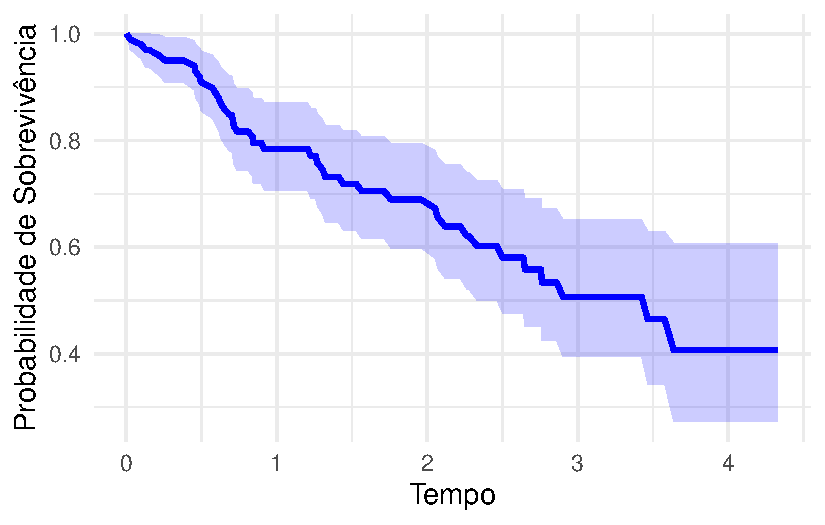
\includegraphics{CII_TEC_N_PARAM_files/figure-pdf/fig-SobrKM-1.pdf}

}

\end{figure}%

\section{Outros Estimadores Não
Parâmetricos}\label{outros-estimadores-nuxe3o-paruxe2metricos}

O estimador de Kaplan-Meier é, indiscutivelmente, o mais utilizado para
estimar \(S(t)\) em análises de sobrevivência. Ele é amplamente
disponibilizado em diversos pacotes estatísticos e abordado em inúmeros
textos de estatística básica. Entretanto, outros dois estimadores de
\(S(t)\) também possuem relevância significativa na literatura
especializada: o estimador de Nelson-Aalen e o estimador da tabela de
vida.

O estimador de Nelson-Aalen, mais recente que o de Kaplan-Meier,
apresenta propriedades similares às deste último. Já o estimador da
tabela de vida possui importância histórica, tendo sido utilizado em
informações derivadas de censos demográficos para estimar
características associadas ao tempo de vida humano. Este estimador foi
inicialmente proposto por demógrafos e atuários no final do século XIX,
sendo empregado principalmente em grandes amostras.

Nesta seção será abordado apenas o estimador de Nelson-Aalen. Para
conhecer mais sobre o estimador da Tabela de Vida ou Tabela Atuarial,
consulte a Seção 2.4.2 do livro \emph{Análise de Sobrevivência Aplicada}
de Colosimo e Giolo (2006).

\subsection{Estimador de Nelson-Aalen}\label{estimador-de-nelson-aalen}

Mais recente que o estimador de Kaplan-Meier, este estimador se baseia
na função de sobrevivência expressa da seguinte forma:

\[
S(t) = \exp\left\{ - \Lambda(t) \right\},
\]

em que \(\Lambda(t)\) é a função de risco acumulado apresentada na
Seção~\ref{sec-TaxaAcu}.

A estimativa para \(\Lambda(t)\) foi inicialmente proposta por Nelson
(1972) posteriormente retomada por Aalen (1978) que demonstrou suas
propriedades assintóticas utilizando processos de contagem. Na
literatura, esse estimador é amplamente conhecido como o estimador de
Nelson-Aalen e é definido pela seguinte expressão:

\begin{equation}\phantomsection\label{eq-ESTNelsonAalen}{
\hat{\Lambda}(t) = \sum_{j:t_{j} < t} \left( \dfrac{d_{j}}{n_{j}} \right),
}\end{equation}

onde \(d_{j}\) e \(n_{j}\) são as mesmas definições usadas no estimador
de Kaplan-Meier. A variância do estimador, conforme proposta por Aalen
(1978), é dada por:

\begin{equation}\phantomsection\label{eq-VarNelsonAalen}{
\hat{Var}(\hat{\Lambda}(t)) = \sum_{j:t_{j} < t} \left( \dfrac{d_{j}}{n_{j}^{2}} \right).
}\end{equation}

Uma alternativa para a estimativa da variância de \(\hat{\Lambda}(t)\),
proposta por Klein (1991), é:

\[
\hat{Var}(\hat{\Lambda}(t)) = \sum_{j:t_{j} < t} \dfrac{(n_{j} - d_{j})d_{j}}{n_{j}^{3}},
\]

entretanto, o estimador da Equação~\ref{eq-VarNelsonAalen} apresenta
menor vício, tornando-o mais preferível que o proposto por Klein (1991).

Desta forma, podemos definir, com base no estimador de Nelson-Aalen, um
estimador para a função de sobrevivência, podendo ser expressa por:

\[
\hat{S}_{NA}(t) = \exp\left\{- \hat{\Lambda}(t) \right\}.
\]

Deve-se, a variância deste estimador, a Aalen e Johansen (1978). Podendo
ser mensurada pela expressão:

\[
\hat{Var}(\hat{S}_{NA}(t)) = \left[ \hat{S}_{NA}(t) \right]^{2} \sum_{j:t_{j} < t} \left( \dfrac{d_{j}}{n_{j}^{2}} \right)
\]

Vale destacar que o estimador de Nelson-Aalen aprenseta, na maioria dos
casos, estimativas próximas ao estimador de Kaplan-Meier. Bohoris (1994)
mostrou que \(\hat{S}_{NA}(t) \geq \hat{S}_{KM}(t)\) para todo \(t\),
isto é, as estimativas obtidas pelo estimador de Nelson-Aalen são
maiores ou iguais às estimativas obtidas pelo estimador de Kaplan-Meier.

\section{Comparação de Curvas de
Sobrevivência}\label{comparauxe7uxe3o-de-curvas-de-sobrevivuxeancia}

Considere um problema na área da saúde em que se deseja comparar dois
grupos: um que receberá tratamento com uma determinada droga e outro que
será o grupo controle. Estatísticas amplamente utilizadas para esse fim
podem ser vistas como generalizações, para dados censurados, de testes
não paramétricos bem conhecidos. Entre esses, o teste \emph{logrank}
(Mantel 1966) é o mais empregado em análises de sobrevivência. Gehan
(1965) propôs uma generalização para a estatística de Wilcoxon. Outras
generalizações foram introduzidas por autores como Peto e Peto (1972) e
Prentice (1978), enquanto Latta (1981) utilizou simulações de Monte
Carlo para comparar diversos testes não-paramétricos.

Nesta seção, será dada ênfase ao teste \emph{logrank}, amplamente
utilizado em análises de sobrevivência e particularmente adequado quando
a razão entre as funções de risco dos grupos a serem comparados é
aproximadamente constante. Ou seja, quando as populações apresentam a
propriedade de riscos proporcionais.

A estatística do teste \emph{logrank} baseia-se na diferença entre o
número observado de falhas em cada grupo e o número esperado de falhas
sob a hipótese nula. Essa abordagem é semelhante à do teste de Mantel e
Haenszel (1959), que combina tabelas de contingência. Além disso, o
teste \emph{logrank} possui a mesma expressão do teste de escore para o
modelo de regressão de Cox, que será apresentado no {[}\ldots{]}. Outros
testes também serão discutidos nesta seção.

Considere, inicialmente, o teste de igualdade entre duas funções de
sobrevivência \(S_{1}(t)\) e \(S_{2}(t)\). Seja
\(t_{1} < t_{2} < \ldots < t_{k}\) a sequência dos tempos de falha
distintos observados na amostra combinada, formada pela união das duas
amostras individuais. Suponha que, no tempo \(t_{j}\), ocorram \(d_{j}\)
falhas e que \(n_{j}\) indivíduos estejam sob risco imediatamente antes
de \(t_{j}\) na amostra combinada. Nas amostras individuais, as
quantidades correspondentes são \(d_{ij}\) e \(n_{ij}\), onde
\(i = 1, 2\) representa o grupo e \(j = 1, \cdots, k\) indica o tempo de
falha.

No tempo \(t_{j}\), os dados podem ser organizados em uma tabela de
contingência \(2 \times 2\), onde \(d_{ij}\) representa o número de
falhas e \(n_{ij} - d_{ij}\) o número de sobreviventes em cada grupo
\(i\). Essa disposição está ilustrada na
Tabela~\ref{tbl-ExampleTableContig}.

\begin{longtable}[]{@{}cccc@{}}

\caption{\label{tbl-ExampleTableContig}Tabela de contingência gerada no
tempo \(t_{j}\).}

\tabularnewline

\toprule\noalign{}
& Grupo 1 & Grupo 2 & \\
\midrule\noalign{}
\endhead
\bottomrule\noalign{}
\endlastfoot
Falha & \(d_{1j}\) & \(d_{2j}\) & \(d_{j}\) \\
Não Falha & \(n_{1j} - d_{1j}\) & \(n_{2j} - d_{2j}\) &
\(n_{j} - d_{j}\) \\
& \(n_{1j}\) & \(n_{2j}\) & \(n_{j}\) \\

\end{longtable}

Condicionado à ocorrência de falhas e censuras até o tempo \(t_{j}\)
(fixando as marginais das colunas) e ao número total de falhas no tempo
\(t_{j}\) (fixando as marginais das linhas), a distribuição de
\(d_{2j}\) é, então, uma hipergeométrica:

\[
\dfrac{ \binom{ n_{1j} }{ d_{1j} } \binom{ n_{2j} }{ d_{2j} } }{ \binom{ n_{j} }{ d_{j} } }.
\]

A média de \(d_{2j}\) é dada por \(w_{2j} = n_{2j} d_{j} n_{j}^{-1}\).
Isso significa que, na ausência de diferenças entre as duas populações
no tempo \(t_{j}\), o número total de falhas (\(d_{j}\)) pode ser
alocado entre as duas amostras proporcionalmente à razão entre o número
de indivíduos sob risco em cada amostra e o número total sob risco.

A variância de \(d_{2j}\) obtida a partir da distribuição
hipergeométrica é:

\[
(V_{j})_{2} = n_{2j}(n_{j} - n_{2j})d_{j}(n_{j} - d_{j}) n_{j}^{-2} (n_{j} - 1)^{-1}.
\]

Portanto, a estatística \(d_{2j} - w_{2j}\) possui média zero e
variância \((V_{j})_{2}\). Se as \(k\) tabelas de contingência forem
independentes, um teste aproximado para avaliar a igualdade entre as
duas funções de sobrevivência pode ser construído com base na seguinte
estatística:

\begin{equation}\phantomsection\label{eq-EstTestelogrank}{
T = \dfrac{ \left[ \sum_{j = 1}^{k} (d_{2j} - w_{2j}) \right]^{2} }{ \sum_{j = 1}^{k} (V_{j})_{2} },
}\end{equation}

que, sob a hipótese nula \(H_{0}: S_{1}(t) = S_{2}(t)\) para todo \(t\)
no período de acompanhamento, segue aproximadamente uma distribuição
qui-quadrado com \(1\) grau de liberdade para amostras grandes.

Para exemplificar a aplicação do teste de \emph{logrank} em dados reais,
utilizou-se o conjunto de dados sobre Leucemia Pediátrica, disponível no
Apêndice (A) do livro \emph{Análise de Sobrevivência Aplicada} de
Colosimo e Giolo (2006). Esses mesmos dados foram usados para gerar a
Figura~\ref{fig-SobrKM}. O objetivo do teste realizado foi avaliar se as
curvas de sobrevivência das categorias da covariável \texttt{r6} são
iguais, com as seguintes hipóteses:

\[
\begin{cases}
  H_{0}: \text{As curvas de sobrevivência dos grupos são iguais ao longo do tempo} \\
  H_{1}: \text{As curvas de sobrevivência dos grupos são diferentes ao longo do tempo.}
\end{cases}
\]

Veja a saída resultante do teste realizado no software R:

\begin{verbatim}
 [1] "leuini" "tempos" "cens"   "idade"  "zpeso"  "zest"   "pas"    "vac"   
 [9] "risk"   "r6"    
\end{verbatim}

\begin{verbatim}
Call:
survdiff(formula = Surv(tempos, cens) ~ grupo, data = dados, 
    rho = 0)

                     N Observed Expected (O-E)^2/E (O-E)^2/V
grupo=Category One  95       34    37.16     0.269      5.73
grupo=Category Zero  8        5     1.84     5.429      5.73

 Chisq= 5.7  on 1 degrees of freedom, p= 0.02 
\end{verbatim}

Ao fixar o nível de significância em 5\% (\(\alpha = 0,05\)), rejeitamos
a hipótese nula. Essa conclusão baseia-se no valor \(p\) (probabilidade
de significância) obtido no teste, calculado como \(p-valor =\)
0.0166441. Como o \(p-valor < \alpha\), rejeita-se \(H_{0}\). Assim,
conclui-se que as curvas de sobrevivência dos grupos são diferentes ao
longo do tempo, ao nível de significância de 5\%.

A generalização do teste \emph{logrank} para a comparação de \(r > 2\)
funções de sobrevivência, \(S_{1}(t), S_{2}(t), \ldots, S_{r}(t)\), é
direta. Utilizando a mesma notação anterior, o índice \(i\) varia agora
de \(1\) a \(r\). Assim, os dados podem ser organizados em uma tabela de
contingência \(2 \times r\), onde cada coluna \(i\) contém \(d_{ij}\)
falhas e \(n_{ij} - d_{ij}\) sobreviventes. Dessa forma, a
Tabela~\ref{tbl-ExampleTableContig} seria estendida para ter \(r\)
colunas em vez de apenas duas.

Condicionada à experiência de falha e censura até o tempo \(t_{j}\) e ao
número total de falhas no tempo \(t_{j}\), a distribuição conjunta de
\(d_{2j}, \ldots,d_{rj}\) segue uma hipergeométrica multivariada, dada
por:

\[
\dfrac{ \prod_{i = 1}^{r} \binom{ n_{ij }}{ d_{ij} } }{ \binom{ n_{j }}{ d_{j} } }.
\]

A média de \(d_{ij}\) é \(w_{ij} = n_{ij} d_{j} n_{j}^{-1}\), bem como a
variância de \(d_{ij}\) e a covariância de \(d_{ij}\) e \(d_{lj}\) são,
respectivamente,

\[
(V_{j})_{ii} = n_{ij} (n_{j} - n_{ij}) d_{j} (n_{j} - d_{j}) n_{j}^{-2} (n_{j} - 1)^{-1}
\]

e

\[
(V_{j})_{il} = - n_{ij} n_{lj} d_{j} (n_{j} - d_{j}) n_{j}^{-2} (n_{j} - 1)^{-1}.
\]

A estatística \(v'_{j} = (d_{2j} - w_{2j}, \ldots, d_{rj} - w_{rj})\)
possui média zero e matriz de variância-covariância \(V_{j}\), com
dimensão \(r - 1\). A matriz \(V_{j}\) contém os termos \((V_{j}){ii}\)
na diagonal principal e \((V_{j})_{il}\), \(i,l = 2, \ldots,r\), fora da
diagonal principal.

A estatística \(v\), que agrega as contribuições de todos os tempos
distintos de falha, é definida como:

\[
v = \sum_{j = 1}^{k} v_{j},
\]

onde \(v\) é um vetor de dimensão \((r - 1) \times 1\), cujos elementos
correspondem às diferenças entre os totais observados e esperados de
falhas.

Considerando, novamente, a independência das \(k\) tabelas de
contingência, a variância de \(v\) é dada por
\(V = V_{1} + \ldots + V_{k}\). Um teste aproximado para a igualdade das
\(r\) funções de sobrevivência pode ser baseado na estatística:

\begin{equation}\phantomsection\label{eq-EstTestelogrankGeneralizado}{
T = v´V^{-1} v,
}\end{equation}

que, sob a hipótese nula \(H_{0}\) (igualdade das curvas de
sobrevivência), segue uma distribuição qui-quadrado com \(r - 1\) graus
de liberdade para amostras grandes. Os graus de liberdade são \(r - 1\)
em vez de \(r\), pois os elementos de \(v\) somam zero.

Uma aplicação para a comparação de \(r\) curvas de sobrevivência
{[}\ldots{]}.

\begin{verbatim}
Código em R a ser preenchido
\end{verbatim}

\subsection{Outros Testes}\label{outros-testes}

{[}\ldots{]}

\bookmarksetup{startatroot}

\chapter{Técnicas Paramétricas - Modelos
Probabilísticos}\label{tuxe9cnicas-paramuxe9tricas---modelos-probabiluxedsticos}

\section{Introdução}\label{introduuxe7uxe3o-2}

No capítulo anterior, foi apresentada uma abordagem não paramétrica para
a análise de dados de sobrevivência, na qual a estimação é realizada sem
assumir uma distribuição de probabilidade específica para o tempo de
sobrevivência.

Os estimadores não paramétricos são derivados diretamente do conjunto de
dados, pressupondo que o mecanismo gerador das informações opera de
maneira distinta em diferentes momentos no tempo, funcionando de forma
quase independente. Assim, conclui-se que a abordagem não paramétrica
possui tantos parâmetros quanto intervalos de tempo considerados.
Contudo, ao incluir covariáveis, o modelo de Kaplan-Meier não permite
estimar diretamente o ``efeito'' dessas covariáveis, limitando-se a
comparar e testar a igualdade entre diferentes curvas de sobrevivência.

Por outro lado, nos modelos de regressão tradicionais, como os modelos
\emph{linear}, \emph{Poisson} ou \emph{logístico}, a escolha de uma
distribuição de probabilidade para a variável resposta \(Y\) e de uma
função para a relação entre \(Y\) e as covariáveis
\(x_{1}, x_{2}, \ldots, x_{p}\) é essencial para identificar o modelo.
Ao aplicar esse conceito na análise de sobrevivência, o tempo até a
ocorrência de um evento de interesse é tratado como a variável resposta.

Nesse contexto, este capítulo introduz uma abordagem paramétrica para
estimar as funções básicas de sobrevivência. Assume-se que a
distribuição de probabilidade do tempo de ocorrência do evento é
conhecida, permitindo a estimação dos parâmetros associados ao modelo de
forma mais estruturada e eficiente.

\section{Distribuições do Tempo de
Sobrevivência}\label{distribuiuxe7uxf5es-do-tempo-de-sobrevivuxeancia}

Seja \(T\) uma variável aleatória que representa o ``tempo de
sobrevivência''. Qual seria a distribuição de probabilidade mais
adequada para representá-la?

Uma característica fundamental da variável aleatória \(T\) é que ela é
contínua e não negativa. Com base nessa propriedade, é possível eliminar
algumas distribuições como candidatas adequadas para modelar \(T\). Por
exemplo, a distribuição normal não é apropriada, pois admite valores
negativos, o que contradiz a natureza do tempo de sobrevivência. Além
disso, os tempos de sobrevivência frequentemente apresentam uma forte
assimetria à direita, reforçando a inadequação da distribuição normal
para esse contexto.

\subsection{Distribuição Exponencial}\label{sec-DistExp}

Se \(T \sim Exp(\alpha)\), a sua função densidade de probabilidade é
expressa da seguinte forma:

\begin{equation}\phantomsection\label{eq-densitExp}{
f(t) = \alpha \exp\{ -\alpha t \}, \ t \geq 0 \ \text{e} \ \alpha > 0.
}\end{equation}

Desta forma, podemos obter a função de sobrevivência com base no
completar da distribuição acumulada de \(T\):

\begin{align*}
    S(t) & = P(T > t) = 1 - P(T \leq t) = 1 - F(t) \\
         & = 1 - [1 - \exp\{ -\alpha t \}] \\
         & = \exp\{ -\alpha t \}.
\end{align*}

Assim definimos, formalmente, a função de sobrevivência como:

\begin{equation}\phantomsection\label{eq-StExp}{
S(t) = \exp\{ -\alpha t \}.
}\end{equation}

Note que o parâmetro \(\alpha\) é a velocidade de queda da função
sobrevivência. Através das relações entre as funções em análise de
sobrevivência, temos a função risco ou taxa de falha. Obtida pela razão
entre da função densidade de probabilidade e a função de sobrevivência:

\begin{equation}\phantomsection\label{eq-RiscoExp}{
\lambda(t) = \dfrac{f(t)}{S(t)} = \dfrac{\alpha \exp\{ -\alpha t \}}{\exp\{ -\alpha t \}} = \alpha = \text{constante}.
}\end{equation}

Sendo a função risco constante para todo tempo observado \(t\), o risco
acumulado é função linear no tempo com uma inclinação da reta dada por
\(\alpha\):

\begin{equation}\phantomsection\label{eq-RiscoAcumExp}{
\Lambda(t) = - \ln[S(t)] = - \ln[ \exp\{ -\alpha t \} ] = - (- \alpha t) = \alpha t
}\end{equation}

Veja, a seguir, a Figura~\ref{fig-CurvasExp} que mostra as curvas de
densidade de probabilidade, de sobrevivência, risco e risco acumulado
para diferentes valores do parâmetro \(\alpha\).

\begin{figure}[H]

\caption{\label{fig-CurvasExp}Funções Densidade de Probabilidade,
Sobrevivência, Risco e Risco Acumulado segundo uma Distribuição
Exponencial para diferentes valores do parâmetro de taxa.}

\begin{minipage}{0.50\linewidth}

\centering{

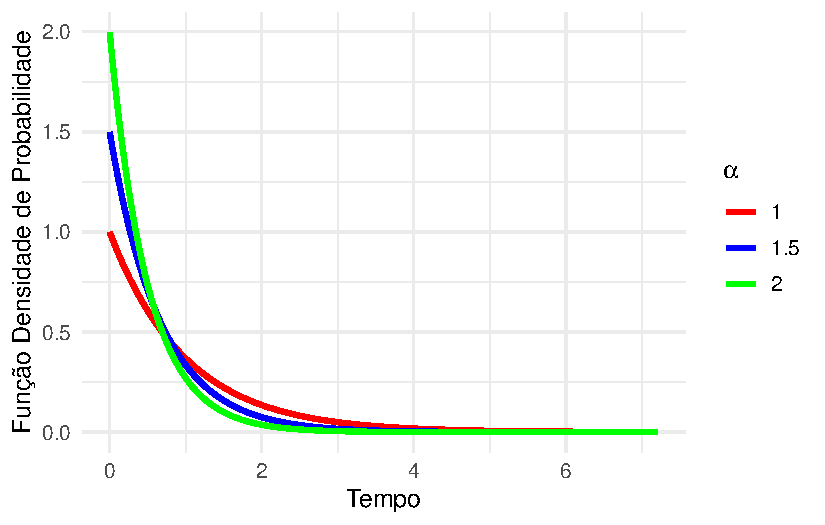
\includegraphics{CIII_TEC_PARAM_files/figure-pdf/fig-CurvasExp-1.pdf}

}

\subcaption{\label{fig-CurvasExp-1}Função Densidade de Probabilidade}

\end{minipage}%
%
\begin{minipage}{0.50\linewidth}

\centering{

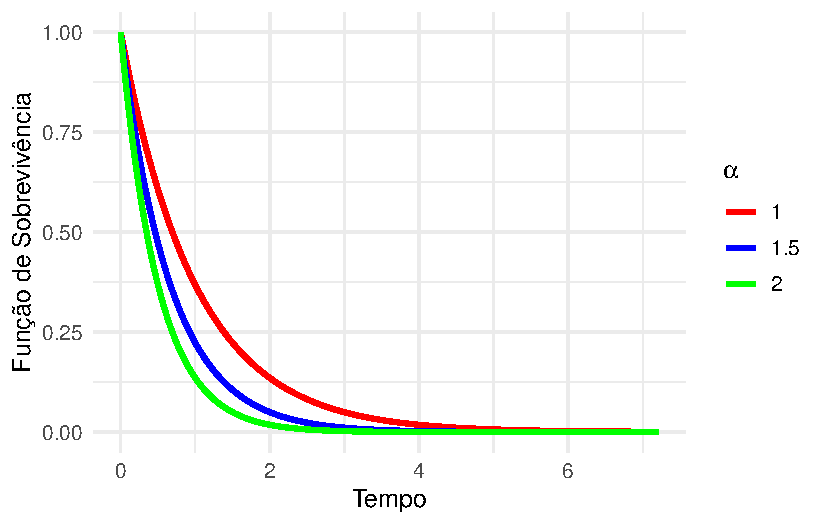
\includegraphics{CIII_TEC_PARAM_files/figure-pdf/fig-CurvasExp-2.pdf}

}

\subcaption{\label{fig-CurvasExp-2}Função de Sobrevivência}

\end{minipage}%
\newline
\begin{minipage}{0.50\linewidth}

\centering{

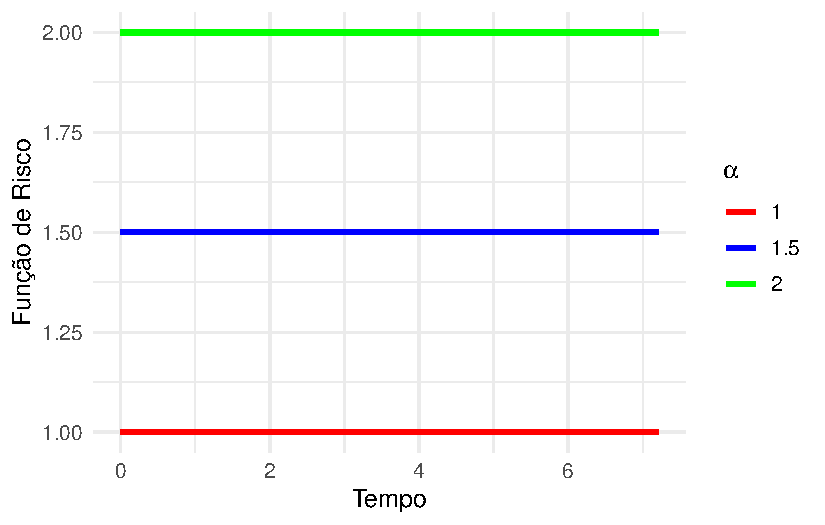
\includegraphics{CIII_TEC_PARAM_files/figure-pdf/fig-CurvasExp-3.pdf}

}

\subcaption{\label{fig-CurvasExp-3}Função de Risco}

\end{minipage}%
%
\begin{minipage}{0.50\linewidth}

\centering{

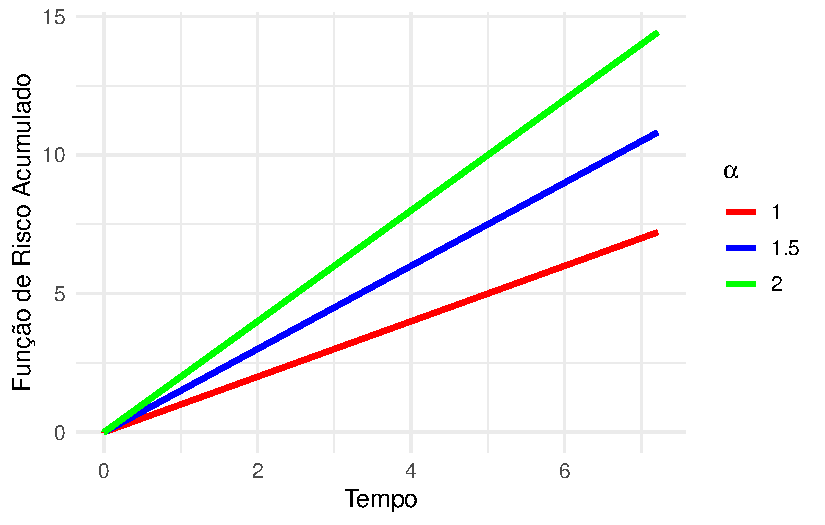
\includegraphics{CIII_TEC_PARAM_files/figure-pdf/fig-CurvasExp-4.pdf}

}

\subcaption{\label{fig-CurvasExp-4}Função de Risco Acumulado}

\end{minipage}%

\end{figure}%

\subsubsection{Algumas considerações}\label{algumas-considerauxe7uxf5es}

Note que, quanto maior o valor de \(\alpha\) (risco), mais abruptamente
a função de sobrevivência \(S(t)\) decresce, e maior é a inclinação da
função de risco acumulado.

A distribuição exponencial, por possuir um único parâmetro, é
matematicamente simples e apresenta um formato assimétrico. Seu uso em
análise de sobrevivência tem uma analogia com a suposição de normalidade
em outras técnicas e áreas da estatística. Entretanto, a suposição de
risco constante associada a essa distribuição é bastante restritiva e,
em muitos casos, pode não ser realista.

Por exemplo, considere um estudo sobre câncer, em que o tempo até o
evento de interesse é definido como o período até a morte ou a cura do
paciente. Para aplicar a distribuição exponencial nesse contexto, seria
necessário assumir que o tempo desde o diagnóstico da doença não afeta a
probabilidade de ocorrência do evento. Essa suposição é delicada, pois o
próprio passar do tempo afeta naturalmente a probabilidade de
sobrevivência, o risco e o risco acumulado, entre outros fatores. Isso
pode ocorrer por causas naturais, como o envelhecimento, que aumenta o
risco com o avanço da idade. Essa característica da distribuição
exponencial é conhecida como falta de memória, o que significa que o
risco futuro é independente do tempo já decorrido.

Quando \(\alpha = 1\), a distribuição é denominada exponencial padrão. A
média e a variância do tempo de sobrevivência, para uma variável que
segue a distribuição exponencial, são expressas como funções inversas do
parâmetro de risco (\(\alpha\)). Assim, quanto maior o risco, menor o
tempo médio de sobrevivência e menor a variabilidade em torno da média.
As expressões são dadas por:

\[
E[T] = \dfrac{1}{\alpha},
\]

\[
Var[T] = \dfrac{1}{\alpha^2}.
\] Como a distribuição de \(T\) é assimétrica, se torna mais usual
utilizar o \emph{tempo mediano de sobrevivência} ao invés de tempo
médio. Pode-se obter o tempo mediano de sobrevivência a partir de um
tempo \(t\), tal que, \(S(t) = 0,5\), logo,

\begin{align*}
    S(t) & = 0,5 \Leftrightarrow \exp\{ -\alpha t \} = 0,5 \Leftrightarrow -\alpha t = \ln(2^{-1}) \\
    \alpha t & = - [-\ln(2)] \Leftrightarrow \alpha t = \ln(2).
\end{align*}

Desta forma, o tempo mediano de sobrevivência é definido como:

\[
T_{mediano} = \dfrac{\ln(2)}{\alpha}.
\]

Em resumo, o modelo exponencial é apropriado para situações em que o
período do experimento é curto o suficiente para que a suposição de
risco constante seja plausível.

\subsection{Distribuição Weibull}\label{sec-DistWeibull}

Na maioria dos casos de análise de sobrevivência na área da saúde, é
mais razoável supor que o risco varia ao longo do tempo, em vez de
permanecer constante.

Atualmente, a \emph{Distribuição Weibull} é amplamente utilizada, pois
permite modelar essa variação do risco ao longo do tempo. Como será
demonstrado, a distribuição exponencial é um caso particular da
distribuição Weibull.

Se o tempo de sobrevivência \(T\) segue uma distribuição Weibull, ou
seja, \(T \sim Weibull(\gamma, \alpha)\), sua função densidade de
probabilidade é dada por:

\begin{equation}\phantomsection\label{eq-densittWei}{
f(t) = \dfrac{ \gamma }{ \alpha^{\gamma} } t^{\gamma - 1} \exp \left\{ - \left( \dfrac{t}{\alpha} \right)^{\gamma} \right\}.
}\end{equation}

A partir da Equação~\ref{eq-densittWei} é possível chegar a função de
sobrevivência da distribuição Weibull sendo está função definida como:

\begin{equation}\phantomsection\label{eq-StWeibull}{
S(t) = \exp \left\{ - \left( \dfrac{t}{\alpha} \right)^{\gamma} \right\},
}\end{equation}

onde \(t \geq 0\), \(\alpha\) o parâmetro escala (ou taxa) e \(\gamma\)
parâmetro de forma. Ambos os parâmetros sempre positivos.

A função de risco, \(\lambda(t)\), depende do tempo de sobrevivência.
Apresentando variação no tempo conforme a expressão:

\begin{equation}\phantomsection\label{eq-RiscoWeibull}{
\lambda (t) = \dfrac{f(t)}{S(t)} = \dfrac{ \gamma }{ \alpha^{\gamma} } t^{\gamma - 1}
}\end{equation}

e a função de risco acumulado da distribuição Weibull é dada por:

\begin{equation}\phantomsection\label{eq-RiscAcumWeibull}{
\Lambda (t) = - \ln[S(t)] = - \ln \left[ \exp \left\{ - \left( \dfrac{t}{\alpha} \right)^{\gamma} \right\} \right] = \left( \dfrac{t}{\alpha} \right)^{\gamma}.
}\end{equation}

Note que, o parâmetro \(\gamma\) determina a forma função de risco da
seguinte maneira:

\begin{itemize}
\tightlist
\item
  \(\gamma < 1 \rightarrow\) função de risco decresce;
\item
  \(\gamma > 1 \rightarrow\) função de risco cresce;
\item
  \(\gamma = 1 \rightarrow\) função de risco constante, caindo no caso
  particular da distribuição exponencial.
\end{itemize}

Veja, a seguir, a Figura~\ref{fig-CurvasWeibull} que mostra as curvas de
densidade, sobrevivência, risco e risco acumulado para diferentes
valores do parâmetro de forma \(\gamma\) e o de escala \(\alpha = 1\).

\begin{figure}[H]

\caption{\label{fig-CurvasWeibull}Funções Densidade de Probabilidade,
Sobrevivência, Risco e Risco Acumulado segundo uma Distribuição Weibull
para diferentes valores do parâmetro de forma.}

\begin{minipage}{0.50\linewidth}

\centering{

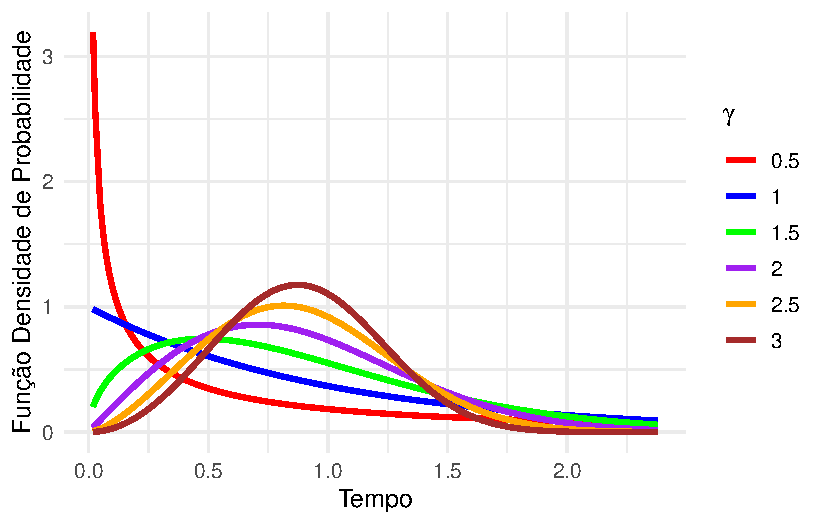
\includegraphics{CIII_TEC_PARAM_files/figure-pdf/fig-CurvasWeibull-1.pdf}

}

\subcaption{\label{fig-CurvasWeibull-1}Função Densidade de
Probabilidade}

\end{minipage}%
%
\begin{minipage}{0.50\linewidth}

\centering{

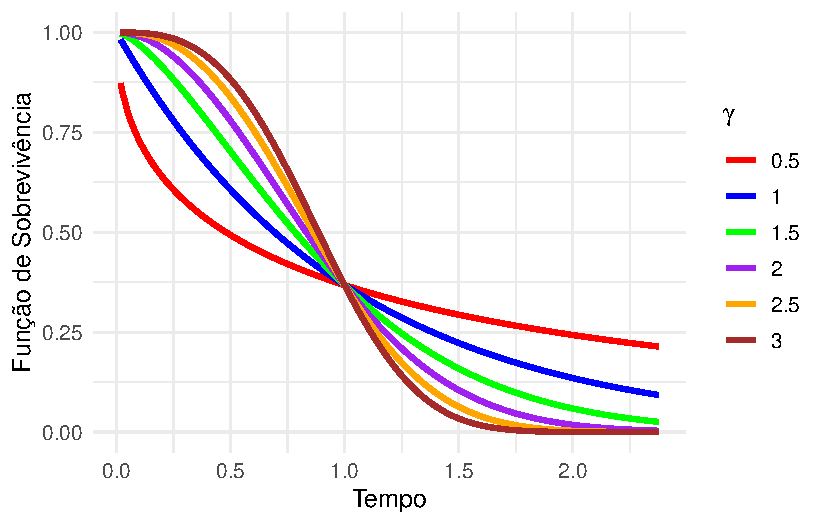
\includegraphics{CIII_TEC_PARAM_files/figure-pdf/fig-CurvasWeibull-2.pdf}

}

\subcaption{\label{fig-CurvasWeibull-2}Função de Sobrevivência}

\end{minipage}%
\newline
\begin{minipage}{0.50\linewidth}

\centering{

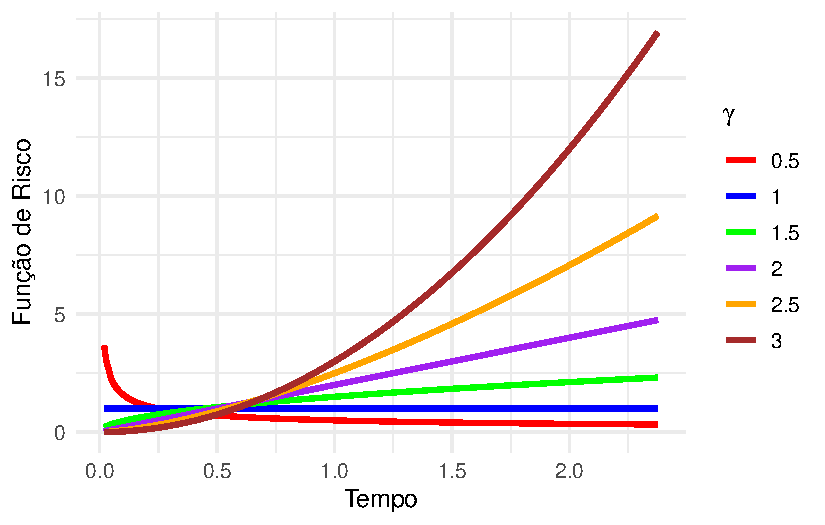
\includegraphics{CIII_TEC_PARAM_files/figure-pdf/fig-CurvasWeibull-3.pdf}

}

\subcaption{\label{fig-CurvasWeibull-3}Função de Risco}

\end{minipage}%
%
\begin{minipage}{0.50\linewidth}

\centering{

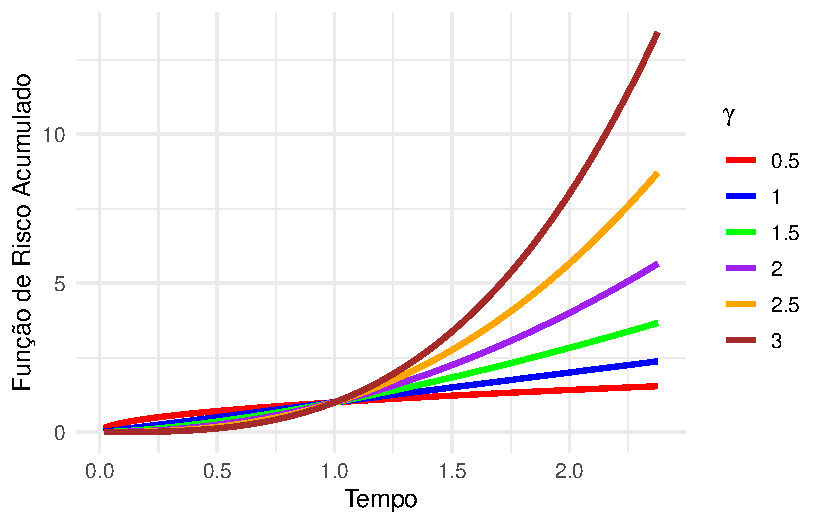
\includegraphics{CIII_TEC_PARAM_files/figure-pdf/fig-CurvasWeibull-4.pdf}

}

\subcaption{\label{fig-CurvasWeibull-4}Função de Risco Acumulado}

\end{minipage}%

\end{figure}%

\subsubsection{Algumas
considerações}\label{algumas-considerauxe7uxf5es-1}

É incluso a função gama na média e variância da distribuição Weibull,
assim,

\[
E[T] = \alpha \Gamma[1 + (1/\gamma)]
\] e

\[
Var[T] = a^{2} \left[ \Gamma [1 + (2/\gamma)] - \Gamma [1 + (1/\gamma)]^{2} \right]
\]

sendo a função gama \(\Gamma [k]\), expressa por
\(\Gamma [k] = \int_{0}^{\infty} t^{k -1} \exp\{t\} dt\).

Afim de se obter o tempo mediano de sobrevivência, igualamos a
probabilidade de sobrevivência a \(0,5\). Desta forma:

\begin{align*}
    S(t) & = 0,5 \Leftrightarrow \exp \left\{ - \left( \dfrac{t}{\alpha} \right)^{\gamma} \right\} = 0,5 \\
    - \left( \dfrac{t}{\alpha} \right)^{\gamma} & = \ln{(2^{-1})} \Leftrightarrow \left( \dfrac{t}{\alpha} \right)^{\gamma} = \ln{(2)} \\
    \dfrac{t}{\alpha} & = [\ln{(2)}]^{1/\gamma}.
\end{align*}

Logo, definimos o tempo mediano de sobrevivência da distribuição Weibull
como:

\[
T_{mediano} = \alpha [\ln{(2)}]^{1/\gamma}.
\]

\subsection{Distribuição
Log-normal}\label{distribuiuxe7uxe3o-log-normal}

Uma outra possibilidade para modelar o tempo de sobrevivência é a
\emph{distribuição Log-normal}. Dizer que
\(T \sim Normal(\mu, \sigma^{2})\) implica em dizer que
\(\ln(T) \sim Log-normal(\mu, \sigma^{2})\) em que \(\mu\) é a média do
logaritmo do tempo de falha e \(\sigma^{2}\) sua variância. Pode-se
fazer uso desta relação para modelar o tempo de sobrevivência conforme
uma distribuição normal, desde que, se aplique o logaritmo aos dados
observados. A função densidade para tal distribuição é dada por:

\begin{equation}\phantomsection\label{eq-densitLognormal}{
f (t) = \dfrac{1}{t \sigma \sqrt{2 \pi}} \exp \left\{- \dfrac{1}{2} \left(\dfrac{\ln(t) - \mu}{\sigma}\right)^{2} \right\}.
}\end{equation}

Assim, quando o tempo de sobrevivência segue uma distribuição
log-normal, sua função de sobrevivência e as demais não tem uma forma
análitica explícita, desde modo, deve-se fazer uso das relações entre as
funções para se obter a função taxa de falha e taxa de falha acumulada.
Desta forma, essas funções são expressas, respectivamente, por:

\begin{equation}\phantomsection\label{eq-StLognormal}{
S (t) = \Phi \left( \dfrac{- \ln(t) + \mu}{\sigma} \right),
}\end{equation}

\[
\lambda (t) = \dfrac{f(t)}{S(t)}
\]

e

\[
\Lambda (t) = - \ln[S(t)]
\]

em que \(\Phi (\cdot)\) é a função de distribuição acumulada da normal
padrão.

Veja a Figura~\ref{fig-CurvasLognormal} que ilustras as curvas usadas na
análise de sobrevivência segundo uma distribuição log-normal, variando o
parâmetro de locação \(\mu\) e fixando o parâmetro de escala
\(\sigma = 1\).

\begin{figure}[H]

\caption{\label{fig-CurvasLognormal}Funções Densidade de Probabilidade,
Sobrevivência, Risco e Risco Acumulado segundo uma Distribuição
Log-normal para diferentes valores do parâmetro de média.}

\begin{minipage}{0.50\linewidth}

\centering{

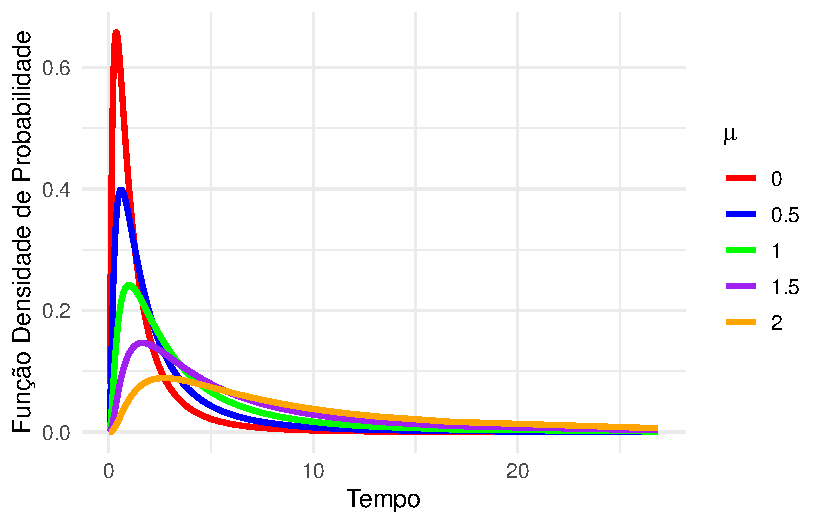
\includegraphics{CIII_TEC_PARAM_files/figure-pdf/fig-CurvasLognormal-1.pdf}

}

\subcaption{\label{fig-CurvasLognormal-1}Função Densidade de
Probabilidade}

\end{minipage}%
%
\begin{minipage}{0.50\linewidth}

\centering{

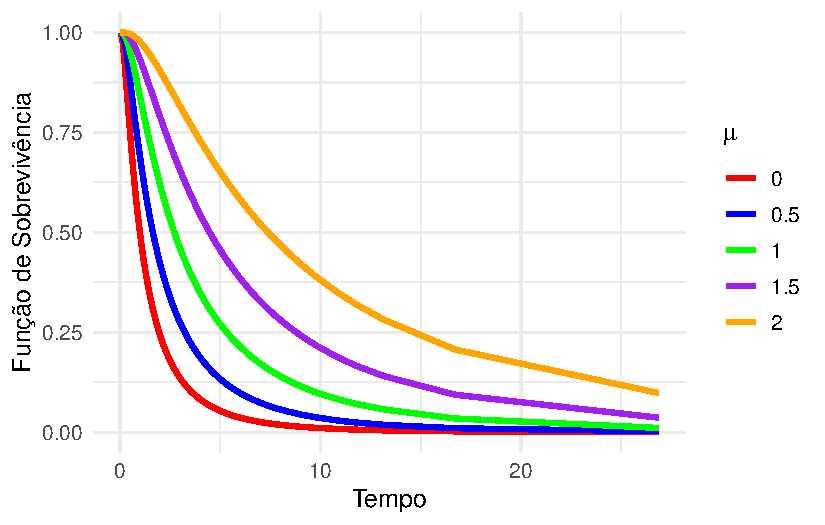
\includegraphics{CIII_TEC_PARAM_files/figure-pdf/fig-CurvasLognormal-2.pdf}

}

\subcaption{\label{fig-CurvasLognormal-2}Função de Sobrevivência}

\end{minipage}%
\newline
\begin{minipage}{0.50\linewidth}

\centering{

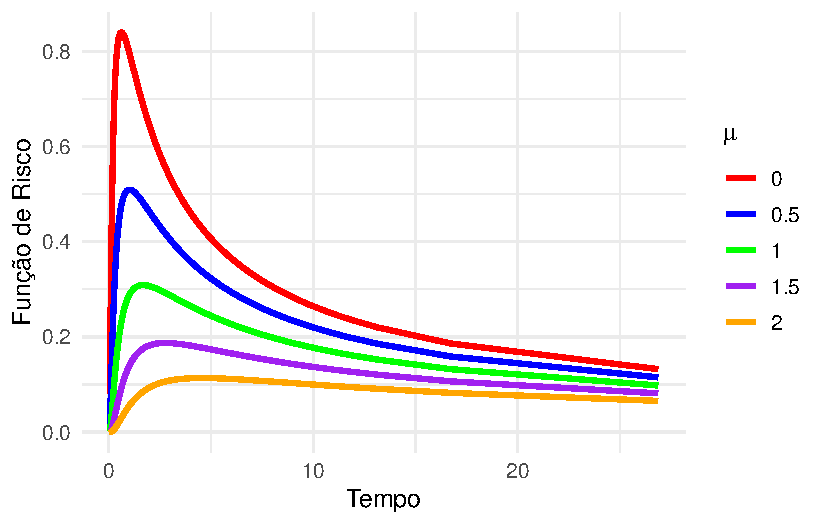
\includegraphics{CIII_TEC_PARAM_files/figure-pdf/fig-CurvasLognormal-3.pdf}

}

\subcaption{\label{fig-CurvasLognormal-3}Função de Risco}

\end{minipage}%
%
\begin{minipage}{0.50\linewidth}

\centering{

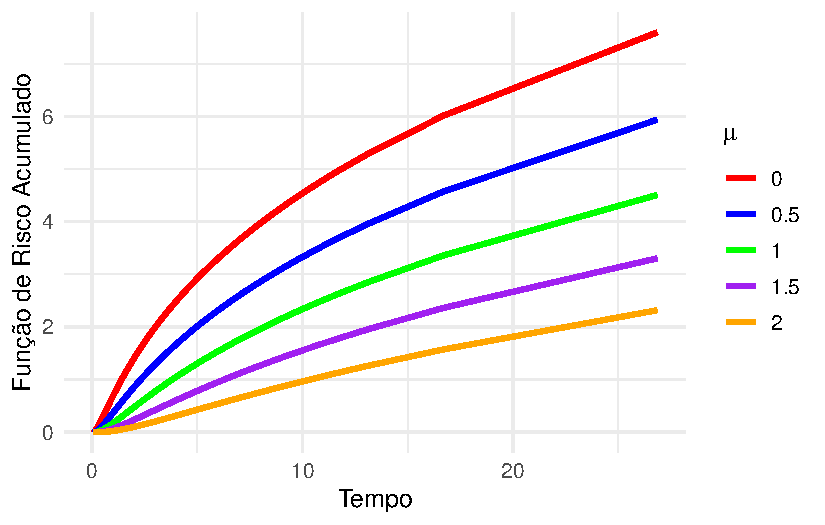
\includegraphics{CIII_TEC_PARAM_files/figure-pdf/fig-CurvasLognormal-4.pdf}

}

\subcaption{\label{fig-CurvasLognormal-4}Função de Risco Acumulado}

\end{minipage}%

\end{figure}%

\subsubsection{Algumas
considerações}\label{algumas-considerauxe7uxf5es-2}

A média e a variância da distribuição log-normal são, respectivamente,
dadas por:

\[
E[T] = \exp\{ \mu + \sigma^{2} / 2 \}
\]

e

\[
Var[T] = \exp\{ 2 \mu + \sigma^{2} \} (\exp\{ \sigma^{2} - 1 \})
\]

\section{Estimação de
Parâmetros}\label{estimauxe7uxe3o-de-paruxe2metros}

Foram apresentados alguns modelos probabilísticos. Esses modelos possuem
quantidades desconhecidas, denominadas \textbf{parâmetros}, ou
\textbf{parâmetro}, quando o modelo depende de uma única quantidade
desconhecida, como no caso da distribuição exponencial.

\subsection{Método de Máxima
Verossimilhança}\label{muxe9todo-de-muxe1xima-verossimilhanuxe7a}

O \emph{Método de Máxima Verossimilhança} baseia-se no princípio de que,
a partir de uma amostra aleatória, a melhor estimativa para o parâmetro
de interesse é aquela que maximiza a probabilidade daquela amostra
observada ter sido observada (Bussab e Morettin 2010).

De forma simples, o método de máxima verossimilhança condensa toda a
informação contida na amostra, por meio da \textbf{função de
verossimilhança}, para encontrar o(s) parâmetro(s) da distribuição que
melhor expliquem os dados. Essa abordagem utiliza o produtório das
densidades \(f(t)\) para cada observação \(t_i\),
\(i = 1, 2, \ldots, n\). Em livros introdutórios de estatística, a
função de verossimilhança é definida da seguinte maneira, para um
parâmetro ou vetor de parâmetros \(\theta\):

\[
L(\theta) = \prod_{i = 1}^{n} f(t_{i}, \theta).
\]

Observe que \(L\) é uma função de \(\theta\), que pode ser um único
parâmetro ou um vetor de parâmetros, como ocorre na distribuição
log-normal, onde \(\theta = (\mu, \sigma^2)\). No entanto, em análise de
sobrevivência, essa definição tradicional de verossimilhança é
insuficiente, pois os dados frequentemente apresentam \textbf{censura},
o que implica que o tempo de falha pode ser apenas parcialmente
observado.

Para lidar com essa característica, utiliza-se a variável indicadora
\(\delta_{i}\), apresentada na Seção~\ref{sec-ReprDados}, que identifica
se o \(i\)-ésimo tempo é um tempo de falha ou de censura. Com base nessa
informação, a função de verossimilhança é ajustada da seguinte forma:

\begin{itemize}
\tightlist
\item
  Para \(\delta_{i} = 1\), o \(i\)-ésimo tempo é um tempo de falha, e
  sua contribuição para \(L(\theta)\) é a densidade de probabilidade
  \(f(t_{i}, \theta)\).
\item
  Para \(\delta_i = 0\), o \(i\)-ésimo tempo é um tempo censurado, e sua
  contribuição para \(L(\theta)\) é a função de sobrevivência
  \(S(t_i)\).
\end{itemize}

Assim, a função de verossimilhança ajustada, que incorpora dados
censurados, é expressa como:

\begin{equation}\phantomsection\label{eq-verossilGeneric}{
L(\theta) = \prod_{i = 1}^{n} \left[ f(t_{i}, \theta) \right]^{\delta_i} \left[ S(t_{i}, \theta) \right]^{1 - \delta_{i}}.
}\end{equation}

Para encontrar o valor de \(\theta\) que maximiza \(L(\theta)\),
utiliza-se a derivada do logaritmo da verossimilhança, igualando-a a
zero:

\[
\frac{\partial \ln [L(\theta)]}{\partial \theta} = 0.
\]

A solução dessa equação fornece o valor de \(\theta\) que maximiza
\(\ln [L(\theta)]\), e consequentemente, \(L(\theta)\).

\subsection{Aplicações no Caso de Não Haver
Censura}\label{aplicauxe7uxf5es-no-caso-de-nuxe3o-haver-censura}

Nesta seção, será demonstrado como determinar o estimador ou os
estimadores de máxima verossimilhança para os parâmetros das
distribuições discutidas.

\subsubsection{Distribuição
Exponencial}\label{distribuiuxe7uxe3o-exponencial}

Considere a distribuição exponencial conforme descrita na
Seção~\ref{sec-DistExp}. O \textbf{Estimador de Máxima Verossimilhança
(EMV)} do parâmetro \(\alpha\) pode ser obtido seguindo os passos
descritos a seguir:

\begin{enumerate}
\def\labelenumi{\arabic{enumi}.}
\tightlist
\item
  Definir a Função de Verossimilhança \(L(\alpha)\):
\end{enumerate}

\begin{align*}
    L (\alpha) & = \prod_{i = 1}^{n} [\alpha \exp \{-\alpha t_{i}\}]^{\delta_{i}} [\exp \{-\alpha t_{i}\}]^{1 - \delta_{i}} \\
               & = \prod_{i = 1}^{n} \alpha^{\delta_{i}} \exp \{ - \alpha t_{i} \}.
\end{align*}

\begin{enumerate}
\def\labelenumi{\arabic{enumi}.}
\setcounter{enumi}{1}
\tightlist
\item
  Tomar o logaritmo da função verossimilhança \(\ln[L(\alpha)]\):
\end{enumerate}

\begin{align*}
    \ln[L (\alpha)] & = \sum_{i = 1}^{n} \ln \left[ \alpha^{\delta_{i}} \exp \{ - \alpha t_{i} \} \right] = \sum_{i = 1}^{n} \ln \left[ \alpha^{\delta_{i}} \right] + \sum_{i = 1}^{n} \ln \left[ \exp \{ - \alpha t_{i} \} \right] \\
                   & = \sum_{i = 1}^{n} \delta_{i} \ln[\alpha] + \sum_{i = 1}^{n} - \alpha t_{i} =  \ln[\alpha] \sum_{i = 1}^{n} \delta_{i} - \alpha \sum_{i = 1}^{n} t_{i}. \\
\end{align*}

\begin{enumerate}
\def\labelenumi{\arabic{enumi}.}
\setcounter{enumi}{2}
\tightlist
\item
  Derivar a função do log da verossimilhança
  \(\dfrac{\partial \ln L (\theta)}{\partial \theta} = 0\):
\end{enumerate}

\begin{align*}
    \dfrac{\partial \ln L (\theta)}{\partial \theta}  & = \dfrac{1}{\alpha} \sum_{i = 1}^{n} \delta_{i} - \sum_{i = 1}^{n} t_{i}.
\end{align*}

\begin{enumerate}
\def\labelenumi{\arabic{enumi}.}
\setcounter{enumi}{3}
\tightlist
\item
  Igualar a derivada a zero e resolver para \(\alpha\):
\end{enumerate}

\begin{align*}
    \dfrac{\partial \ln L (\theta)}{\partial \theta}  & = 0 \\
    \dfrac{1}{\hat{\alpha}} \sum_{i = 1}^{n} \delta_{i} - \sum_{i = 1}^{n} t_{i} & = 0 \\
    \hat{\alpha} & = \dfrac{\sum_{i = 1}^{n} \delta_{i}}{\sum_{i = 1}^{n} t_{i}}
\end{align*}

Note que, para o caso em que não se tem censura o numerador,
\(\sum_{i = 1}^{n} \delta_{i}\), equivale ao tamanho da amostra \(n\).
Logo, o EMV para \(\alpha\) no caso de não haver censura nos dados é:

\[
\hat{\alpha} = \dfrac{n}{\sum_{i = 1}^{n} t_{i}}
\]

Simulou-se uma amostra proveniente de uma distribuição exponencial e, a
partir dessa amostra, obteve-se a estimativa de máxima verossimilhança
(EMV) para o parâmetro \(\alpha\). Veja a Tabela~\ref{tbl-EMVexpSt}, que
apresenta as dez primeiras observações e suas respectivas funções de
sobrevivência real e estimada.

\begin{longtable}[]{@{}ccc@{}}

\caption{\label{tbl-EMVexpSt}Comparação da dez primeiras observações
entre o valor Real e Estimado da Função de Sobrevivência.}

\tabularnewline

\toprule\noalign{}
Tempo & \(S(t)\) & \(\hat{S}(t)\) \\
\midrule\noalign{}
\endhead
\bottomrule\noalign{}
\endlastfoot
0.0006 & 0.9992 & 0.9992 \\
0.0009 & 0.9987 & 0.9987 \\
0.0029 & 0.9956 & 0.9958 \\
0.0031 & 0.9954 & 0.9955 \\
0.0032 & 0.9952 & 0.9953 \\
0.0038 & 0.9944 & 0.9946 \\
0.0039 & 0.9942 & 0.9944 \\
0.0042 & 0.9937 & 0.9938 \\
0.0053 & 0.9921 & 0.9924 \\
0.0060 & 0.9910 & 0.9913 \\

\end{longtable}

O valor verdadeiro do parâmetro é \(\alpha =\) 1.5. A estimativa de
máxima verossimilhança obtida foi \(\hat{\alpha} =\) 1.46. Na
Figura~\ref{fig-CompEMVexp}, comparamos graficamente as duas curvas de
sobrevivência, ilustrando o valor real do parâmetro \(\alpha\) e sua
estimativa \(\hat{\alpha}\).

\begin{figure}[H]

\caption{\label{fig-CompEMVexp}Comparação do verdadeiro valor do
parâmetro \(\alpha\) com sua estimativa de máxima verossimilhança.}

\centering{

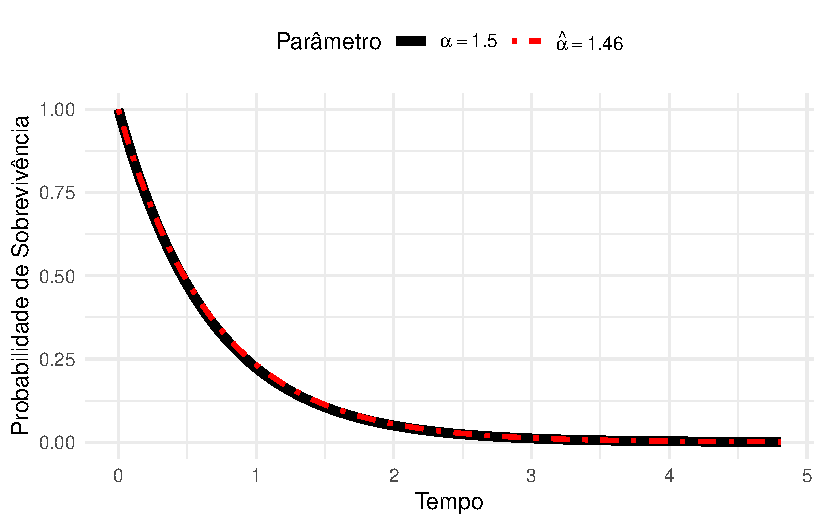
\includegraphics{CIII_TEC_PARAM_files/figure-pdf/fig-CompEMVexp-1.pdf}

}

\end{figure}%

\subsubsection{Distribuição Weibull}\label{distribuiuxe7uxe3o-weibull}

Para a distribuição Weibull, apresentada na Seção~\ref{sec-DistWeibull},
não há uma forma analítica para as estimativas de máxima verossimilhança
dos parâmetros \(\gamma\) (forma) e \(\alpha\) (escala). Assim, a
obtenção dessas estimativas depende de métodos numéricos, sendo o
\textbf{Método Iterativo de Newton-Raphson} uma abordagem amplamente
utilizada.

O Método de Newton-Raphson é um procedimento iterativo eficiente para
resolver equações não lineares, muito empregado na estimação de
parâmetros estatísticos. No ajuste de distribuições, como a Weibull no
contexto de análise de sobrevivência, o método busca maximizar a função
de verossimilhança resolvendo o sistema de equações derivado das
condições de otimalidade (gradiente nulo).

A fórmula iterativa é:

\[
\theta_{n+1} = \theta_{n} - \mathbf{H}^{-1}(\theta_{n}) \nabla L(\theta_{n}),
\]

onde:

\begin{itemize}
\tightlist
\item
  \(\theta_{n}\) é o vetor de parâmetros estimados na iteração \(n\);
\item
  \(L(\theta)\) é a função log-verossimilhança;
\item
  \(\nabla L(\theta)\) é o vetor gradiente, contendo as derivadas
  parciais de \(L(\theta)\) em relação aos parâmetros;
\item
  \(\mathbf{H}(\theta)\) é a matriz Hessiana, composta pelas segundas
  derivadas de \(L(\theta)\).
\end{itemize}

\textbf{Vantagens no ajuste de distribuições:}

\begin{itemize}
\tightlist
\item
  \textbf{Eficiência}: O método apresenta convergência rápida quando o
  ponto inicial \(\theta_{0}\) está próximo dos valores reais dos
  parâmetros.
\item
  \textbf{Flexibilidade}: Pode ser aplicado a diversos modelos
  probabilísticos, incluindo a Weibull, que é amplamente utilizada para
  modelar tempos de vida e dados de sobrevivência.
\end{itemize}

\textbf{Cuidados na aplicação:}

\begin{itemize}
\tightlist
\item
  \textbf{Convergência}: A convergência do método não é garantida caso o
  ponto inicial esteja muito distante da solução ou se as condições de
  regularidade do modelo não forem atendidas.
\item
  \textbf{Cálculo da Hessiana}: O cálculo da matriz Hessiana pode ser
  computacionalmente custoso, especialmente em distribuições com maior
  complexidade.
\end{itemize}

No caso da distribuição Weibull, a aplicação do método Newton-Raphson
requer o cálculo das derivadas em relação aos parâmetros \(\gamma\) e
\(\alpha\), permitindo ajustar o modelo aos dados observados de tempos
de sobrevivência de forma precisa e eficiente.

O Método Iterativo de Newton-Raphson pode ser implementado de duas
formas principais:

\begin{enumerate}
\def\labelenumi{\arabic{enumi}.}
\tightlist
\item
  \textbf{Construção Algorítmica Manual:} Consiste na definição e
  cálculo explícito das funções necessárias, como a função de
  verossimilhança, o gradiente e a Hessiana.
\item
  \textbf{Uso da Função \texttt{optim} no R:} Esta função automatiza o
  processo de otimização e oferece uma implementação flexível e
  eficiente.
\end{enumerate}

Para um melhor entendimento do Método Iterativo de Newton-Raphson veja o
Apêndice (D) do livro \emph{Análise de Sobrevivência Aplicada} de
Colosimo e Giolo (2006).

A seguir, será apresentada a construção do algoritmo passo a passo.
Começa-se definindo a função de verossimilhança para a distribuição
Weibull, que pode ser obtida a partir da
Equação~\ref{eq-verossilGeneric} substituindo a função densidade e a
função de sobrevivência específicas da distribuição Weibull. Assim:

\begin{align*}
    L (\gamma, \alpha) & = \prod_{i = 1}^{n} \left[ \dfrac{\gamma}{\alpha^{\gamma}} t_{i}^{\gamma - 1} \exp \left\{ - \left(\dfrac{t_{i}}{\alpha}\right)^{\gamma} \right\} \right]^{\delta_{i}} \left[ \exp \left\{ - \left(\dfrac{t_{i}}{\alpha}\right)^{\gamma} \right\} \right]^{1 - \delta_{i}} \\
    & = \prod_{i = 1}^{n} \left[ \dfrac{\gamma}{\alpha^{\gamma}} t_{i}^{\gamma - 1} \right]^{\delta_{i}}  \exp \left\{ - \left(\dfrac{t_{i}}{\alpha}\right)^{\gamma} \right\}.
\end{align*}

Toma-se o logaritmo de \(L(\gamma, \alpha)\), logo:

\begin{align*}
    \ln[L(\gamma, \alpha)] & = \sum_{i = 1}^{n} \delta_{i} \ln[\gamma] - \sum_{i = 1}^{n} \delta_{i} \gamma \ln[\alpha] + \sum_{i = 1}^{n} \delta_{i} (\gamma - 1) \ln[t_{i}] + \sum_{i = 1}^{n} - (\alpha^{-1} t_{i})^{\gamma} \\
    & = \ln[\gamma] \sum_{i = 1}^{n} \delta_{i} - \gamma \ln[\alpha] \sum_{i = 1}^{n} \delta_{i} + (\gamma - 1) \sum_{i = 1}^{n} \delta_{i} \ln[t_{i}] + \sum_{i = 1}^{n} - (\alpha^{-1} t_{i})^{\gamma}.
\end{align*}

Agora, aplica-se as derivadas de primeira ordem em relação a \(\gamma\)
e \(\alpha\).

\[
\dfrac{\partial \ln[L(\gamma, \alpha)]}{\partial \gamma} = \dfrac{1}{\gamma} \sum_{i = 1}^{n} \delta_{i} - \ln[\alpha] \sum_{i = 1}^{n} \delta_{i} + \sum_{i = 1}^{n} \delta_{i} \ln[t_{i}] - \sum_{i = 1}^{n} (\alpha^{-1} t_{i})^{\gamma} \ln[\alpha^{-1} t_{i}]
\]

\[
\dfrac{\partial \ln[L (\gamma, \alpha)]}{\partial \alpha} = - \dfrac{\gamma}{\alpha} \sum_{i = 1}^{n} \delta_{i} + \gamma \alpha^{-\gamma - 1} \sum_{i = 1}^{n} t_{i}^{\gamma}
\]

Toma-se agora as derivadas de segunda ordem.

\[
\dfrac{\partial^{2} \ln[L (\gamma, \alpha)]}{\partial \gamma^{2}} =  - \dfrac{1}{\gamma^{2}} \sum_{i = 1}^{n} \delta_{i} - \sum_{i = 1}^{n} (\alpha^{-1} t_{i})^{\gamma} (\ln[\alpha^{-1} t_{i}])^{2}
\]

\[
\dfrac{\partial^{2} \ln [L(\gamma, \alpha)]}{\partial \alpha^{2}} = - \dfrac{\gamma}{\alpha^{2}} \sum_{i = 1}^{n} \delta_{i} - \gamma (\gamma + 1) \alpha^{-\gamma - 2} \sum_{i = 1}^{n} t_{i}^{\gamma}
\]

\[
\dfrac{\partial^{2} \ln[L(\gamma, \alpha)]}{\partial \gamma \partial \alpha} = \dfrac{\partial^{2} \ln[L(\gamma, \alpha)]}{\partial \alpha \partial \gamma} = - \dfrac{1}{\alpha} \sum_{i = 1}^{n} \delta_{i} + \alpha^{- \gamma - 1} \sum_{i = 1}^{n} t_{i}^{\gamma} \left( \gamma \ln\left[ \dfrac{t_{i}}{\alpha} \right] + 1 \right)
\]

Com todas as derivadas definidas, pode-se construir o algoritmo
iterativo de Newton-Raphson. Veja a saída obtida à implementação do
algoritmo de Newton-Raphson escrito pelo autor.

\begin{verbatim}
Número de Iterações Necessárias: 46 
\end{verbatim}

\begin{verbatim}
Estimativa para o parâmetro de forma: 2.015515 
\end{verbatim}

\begin{verbatim}
Estimativa para o parâmetro de forma: 1.507206 
\end{verbatim}

O mesmo resultado, ou bem próximo, pode ser obtido de uma forma mais
direta por meio do uso da função \texttt{optim} para otimização. Veja a
saída obtida de tal função.

\begin{verbatim}
O método convergiu? TRUE 
\end{verbatim}

\begin{verbatim}
Estimativa para o parâmetro de forma: 2.015526 
\end{verbatim}

\begin{verbatim}
Estimativa para o parâmetro de escala: 1.507207 
\end{verbatim}

Assim como na distribuição exponencial, será feita uma comparação entre
o real e estimado. Veja a Tabela~\ref{tbl-EMVweibullSt} que mostra as
dez primeiras observações e suas respectivas funções de sobrevivência,
sobrevivência real e sobrevivência estimada.

\begin{longtable}[]{@{}ccc@{}}

\caption{\label{tbl-EMVweibullSt}Real e Estimado para as Funções de
Sobrevivência da Distribuição Weibull}

\tabularnewline

\toprule\noalign{}
Tempo & \(S(t)\) & \(\hat{S}(t)\) \\
\midrule\noalign{}
\endhead
\bottomrule\noalign{}
\endlastfoot
0.0006 & 0.9992 & 0.9992 \\
0.0009 & 0.9987 & 0.9987 \\
0.0029 & 0.9956 & 0.9958 \\
0.0031 & 0.9954 & 0.9955 \\
0.0032 & 0.9952 & 0.9953 \\
0.0038 & 0.9944 & 0.9946 \\
0.0039 & 0.9942 & 0.9944 \\
0.0042 & 0.9937 & 0.9938 \\
0.0053 & 0.9921 & 0.9924 \\
0.0060 & 0.9910 & 0.9913 \\

\end{longtable}

Temos também a comparação dessas duas curvas de sobrevivência,
ilustradas na Figura~\ref{fig-CompEMVWeibull}.

\begin{figure}[H]

\caption{\label{fig-CompEMVWeibull}Comparação do verdadeiro valor dos
parâmetros \(\gamma\) e \(\alpha\) com suas estimativas de máxima
verossimilhança.}

\centering{

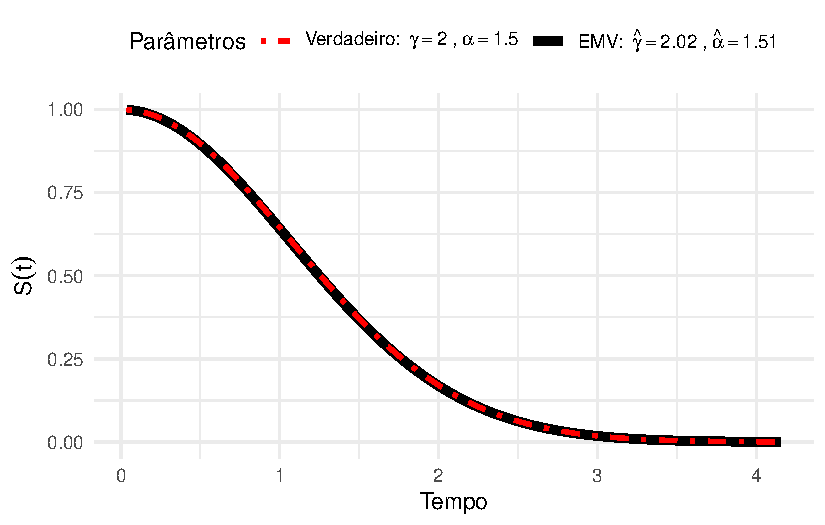
\includegraphics{CIII_TEC_PARAM_files/figure-pdf/fig-CompEMVWeibull-1.pdf}

}

\end{figure}%

\subsection{Aplicação caso haja
Censura}\label{aplicauxe7uxe3o-caso-haja-censura}

Amostras aleatórias foram geradas simultaneamente a partir das
distribuições Weibull e Exponencial, com o objetivo de modelar tempos de
falha e censura, respectivamente. Para cada unidade amostral, o tempo
observado foi definido como a menor realização entre as duas
distribuições, ou seja: \[
t_{i} = min(T_{i}, C_{i}),
\]

onde

\begin{itemize}
\tightlist
\item
  \(T \sim Weibull(\gamma, \alpha)\) representa o tempo real de falha,
  assumindo uma distribuição Weibull parametrizada por forma
  (\(\gamma = 2\)) e escala (\(\alpha = 1.5\));
\item
  \(C \sim Exp(\alpha)\) corresponde ao tempo de censura, assumindo uma
  distribuição Exponencial com parâmetro de taxa \(\alpha = 1\).
\end{itemize}

A censura ocorre quando o tempo de observação não corresponde ao tempo
real de falha, ou seja, quando \(C_{i} < T_{i}\). Nesse caso, o evento
de interesse não foi completamente observado, sendo conhecido apenas que
o verdadeiro tempo de falha excede o valor registrado. Essa
característica, fundamental na análise de sobrevivência, requer métodos
estatísticos específicos para garantir inferências adequadas a partir de
dados censurados.

\begin{longtable}[]{@{}cc@{}}

\caption{\label{tbl-DATASIMULCENS}Dados de Sobrevivência Simulados com
Tempos de Falha Censurados.}

\tabularnewline

\toprule\noalign{}
Tempo & Censura \\
\midrule\noalign{}
\endhead
\bottomrule\noalign{}
\endlastfoot
0.4031 & 1 \\
0.3391 & 1 \\
0.1110 & 0 \\
1.1015 & 1 \\
0.6505 & 1 \\
0.6842 & 1 \\
0.1960 & 1 \\
0.5747 & 0 \\
0.5934 & 0 \\
0.5528 & 0 \\

\end{longtable}

Foram simulados 1000 tempos de falha, dentre eles, 50.6 são tempos de
falha censurados. Deixa-se uma sugestão de variar essa proporção e
avaliar a qualidade das estimativas. De posse dos dados simulados,
gerou-se a Figura~\ref{fig-HistSimulCens}.

\begin{figure}[H]

\caption{\label{fig-HistSimulCens}Histograma dos dados simulados.}

\centering{

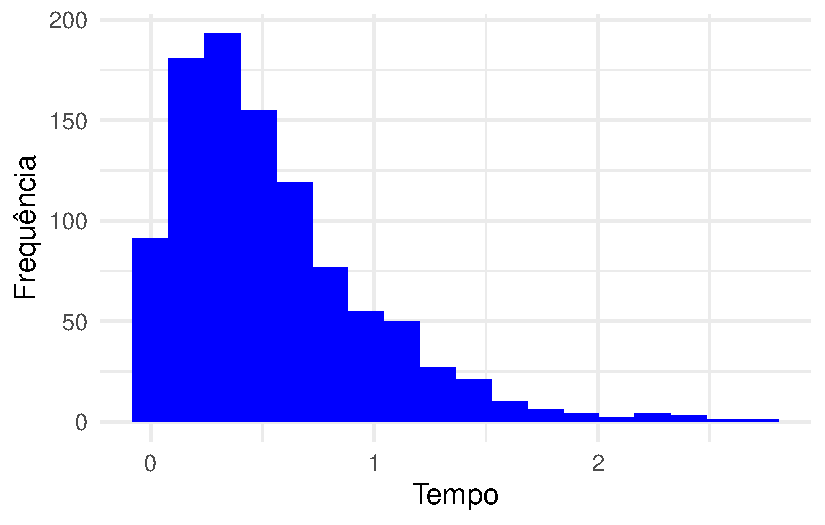
\includegraphics{CIII_TEC_PARAM_files/figure-pdf/fig-HistSimulCens-1.pdf}

}

\end{figure}%

Estimou-se a curva de sobrevivência pelo estimador de Kaplan-Meier,
segundo uma distribuição exponencial e segundo uma distribuição Weibull.
A Figura~\ref{fig-CompCurvSobr} mostra a comparação dessas estimativas.

\begin{figure}[H]

\caption{\label{fig-CompCurvSobr}Comparação das Curvas de Sobrevivência
de Kaplan-Meier, Modelo Exponencial e Modelo Weibull.}

\centering{

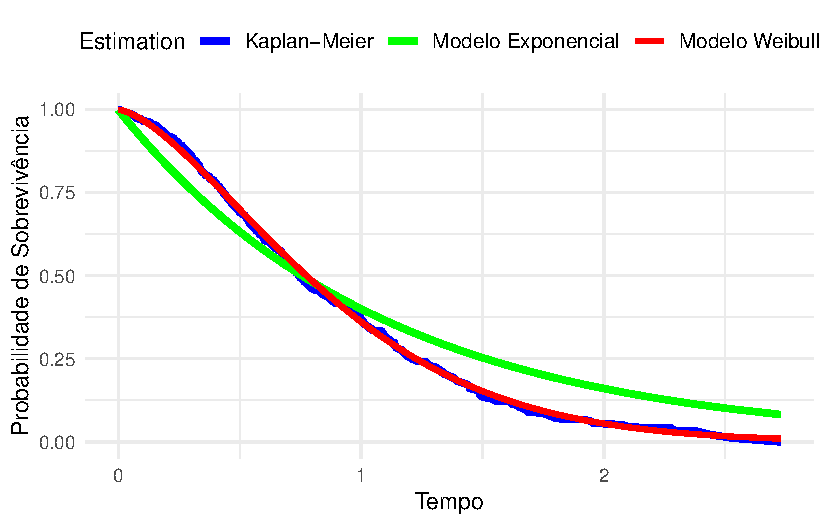
\includegraphics{CIII_TEC_PARAM_files/figure-pdf/fig-CompCurvSobr-1.pdf}

}

\end{figure}%

{[}\ldots{]}

\bookmarksetup{startatroot}

\chapter{Modelos de Tempo de Vida
Acelerado}\label{modelos-de-tempo-de-vida-acelerado}

\section{Introdução}\label{introduuxe7uxe3o-3}

No capítulo anterior, foram apresentados modelos paramétricos para dados
de sobrevivência. Entretanto, esses modelos não contemplam a inclusão de
covariáveis na análise do tempo de sobrevivência. Neste capítulo,
exploraremos esse método.

No modelo de regressão linear clássico, a relação entre a variável
resposta \(Y\) e as covariáveis \(\mathbf{x'}\) é aditiva, ou seja,
mudanças nas covariáveis alteram \(Y\) de maneira linear. O modelo de
regressão linear clássico é expresso como:

\begin{equation}\phantomsection\label{eq-LinearModel}{
Y = \beta_{0} + \beta_{1} X_{1} + \beta_{2} X_{2} \ldots + \beta_{p} X_{p} + \varepsilon,
}\end{equation}

onde \(\varepsilon\) é a parte estocástica (erro) que segue uma
distribuição \(Normal(0, \sigma^{2})\).

No entanto, em análise de sobrevivência, essa suposição não se sustenta,
pois o efeito das covariáveis geralmente acelera ou retarda o tempo de
falha, tornando necessária uma abordagem multiplicativa. Este modelo de
regressão é chamado de Modelo de \emph{Tempo de Vida Acelerado}
(Accelerated Failure Time - AFT).

No modelo AFT, assume-se que o tempo de falha \(T\) é afetado por um
fator de aceleração exponencial das covariáveis. Esse fator
multiplicativo indica se o tempo até o evento será prolongado ou
encurtado. Assim, o modelo é definido como:

\begin{equation}\phantomsection\label{eq-RelationAFT}{
T = \exp\{ \mathbf{x'} \boldsymbol{\beta} \} \varepsilon = \exp\{ \beta_{0} + \beta_{1} X_{1} + \beta_{2} X_{2} \ldots + \beta_{p} X_{p} \} \varepsilon,
}\end{equation}

onde \(\varepsilon\) é um termo de erro multiplicativo que captura a
variabilidade não explicada pelas covariáveis. Aplicando a transformação
logarítmica em \(T\) obtém-se a forma linearizável de
Equação~\ref{eq-RelationAFT} que aproxima-se da
Equação~\ref{eq-LinearModel}, de forma que

\[
\ln[T] = \beta_{0} + \beta_{1} X_{1} + \beta_{2} X_{2} \ldots + \beta_{p} X_{p} + v,
\]

onde \(v = \ln[\varepsilon]\) segue uma distribuição de valor extremo.
Essa escolha para a distribuição dos erros decorre do fato de que os
tempos de sobrevivência frequentemente apresentam forte assimetria à
direita. Portanto, os erros não podem ser adequadamente representados
por uma distribuição normal, sendo mais apropriado assumir distribuições
como Log-normal, Weibull ou Exponencial.

Nos modelos AFT, a função de sobrevivência sofre um ajuste devido ao
efeito das covariáveis, que podem acelerar ou retardar o tempo de falha.
Assim, a função de sobrevivência condicional às covariáveis é expressa
como:

\begin{equation}\phantomsection\label{eq-fSobrAFT}{
S (t | x) = P (T > t / \exp\{ \mathbf{x'} \boldsymbol{\beta}\}).
}\end{equation}

Como o tempo de falha é ajustado pelo fator de aceleração, a função de
risco também precisa ser reformulada para incorporar o efeito das
covariáveis. A forma geral da função de risco em modelos AFT é dada por:

\begin{equation}\phantomsection\label{eq-fhazardAFT}{
\lambda(t | \mathbf{x}) = \lambda_{0}(t) g(\mathbf{x}).
}\end{equation}

Nesta expressão, \(\lambda_{0}(t)\), representa a função de risco basal,
isto é, representa o risco no tempo \(t\) quando todas as covariáveis
são iguais a zero, ou seja, na ausência de efeitos das covariáveis. Já o
termo \(g(\mathbf{x}) = \exp\{ - \mathbf{x'} \boldsymbol{\beta} \}\) age
como um fator de ajuste, mensurando o impacto das covariáveis na taxa de
falha.

\section{Modelo Exponencial}\label{modelo-exponencial}

Em modelos AFT, a função de sobrevivência à distribuição exponencial é
expressa por:

\begin{equation}\phantomsection\label{eq-AFTexpSt}{
S (t | x) = \exp \left\{- \alpha \left( \dfrac{t}{\exp\{ \mathbf{x'} \boldsymbol{\beta} \}} \right) \right\}.
}\end{equation}

Com função de risco dada por:

\begin{equation}\phantomsection\label{eq-AFTexpht}{
\lambda(t | \mathbf{x}) = \alpha \exp\{ - \mathbf{x'} \boldsymbol{\beta} \}.
}\end{equation}

\section{Distribuição Weibull}\label{distribuiuxe7uxe3o-weibull-1}

Para modelos AFT, baseados na distribuição Weibull, a função de
sobrevivência é dada por:

\begin{equation}\phantomsection\label{eq-AFTweibSt}{
S (t | x) = \exp \left\{ - \left( \dfrac{t}{\alpha \exp\{ - \mathbf{x'} \boldsymbol{\beta} \} } \right)^{\gamma} \right\}.
}\end{equation}

Assim, pode-se escrever a função de risco da distribuição Weibull como:

\begin{equation}\phantomsection\label{eq-AFTeeibht}{
\lambda(t | \mathbf{x}) = \dfrac{ \gamma }{ \alpha^{\gamma} } t^{\gamma - 1} \exp\{ - \mathbf{x'} \boldsymbol{\beta} \}
}\end{equation}

\section{Distribuição Exponencial por
Partes}\label{distribuiuxe7uxe3o-exponencial-por-partes}

{[}\ldots{]}

\section{Estimação de
Parâmetros}\label{estimauxe7uxe3o-de-paruxe2metros-1}

Assim como no capítulo anterior, a estimação dos parâmetros será
realizada pelo método de máxima verossimilhança. Recordando que a função
de verossimilhança para dados censurados é expressa como:

\begin{align*}
L(\theta) & = \prod_{i = 1}^{n} \left[f(t_{i} | \mathbf{x}) \right]^{\delta_{i}} \left[S(t_{i} | \mathbf{x}) \right]^{1 - \delta_{i}} \\
          & = \prod_{i = 1}^{n} \left[\lambda(t_{i} | \mathbf{x}) \right]^{\delta_{i}} S(t_{i} | \mathbf{x}),
\end{align*}

onde:

\begin{itemize}
\tightlist
\item
  \(\delta_{i}\) é a variável indicadora, assumindo \(1\) se \(t_{i}\)
  for um tempo de falha observado e \(0\) se for censurado;
\item
  \(f(t_{i}|\mathbf{x})\) representa a função densidade de probabilidade
  condicional;
\item
  \(S(t_{i}|\mathbf{x})\) é a função de sobrevivência condicional;
\item
  \(\lambda(t_{i}|\mathbf{x})\) corresponde à função de risco
  condicional.
\end{itemize}

O estimador de máxima verossimilhança (EMV) para \(\theta\) é obtido
maximizando a função de log-verossimilhança, dada por:

\[
\ln{L(\theta)} = \sum_{i = 1}^{n} \delta_{i} \ln{\lambda(t_{i}|\mathbf{x})} + \ln{S(t_{i}|\mathbf{x})}.
\]

Portanto, o parâmetro ou o conjunto de parâmetros \(\theta\) que
maximiza \(\ln{L(\theta)}\) representa a melhor estimativa para a
amostra observada, sendo obtido por métodos numéricos como o
Newton-Raphson.

\section{Implementação
Computacional}\label{implementauxe7uxe3o-computacional}

\subsection{Distribuição
Exponencial}\label{distribuiuxe7uxe3o-exponencial-1}

\subsubsection{Geração dos Dados}\label{gerauxe7uxe3o-dos-dados}

\begin{itemize}
\tightlist
\item
  \textbf{Funções de Geração:}
\end{itemize}

\begin{itemize}
\tightlist
\item
  \textbf{Simulação dos dados:}
\end{itemize}

Veja a Tabela~\ref{tbl-SIMULexpAFT} que apresenta as dez primeiras
observações simuladas.

\begin{longtable}[]{@{}ccccc@{}}

\caption{\label{tbl-SIMULexpAFT}Dez primeiras observações Simuladas para
Dados de Sobrevivência Censurados baseados no Modelo Exponencial.}

\tabularnewline

\toprule\noalign{}
Tempo & Delta & Constante & X1 \textasciitilde{} Bern(0,5) & X2
\textasciitilde{} Normal(0, 1) \\
\midrule\noalign{}
\endhead
\bottomrule\noalign{}
\endlastfoot
0.5804 & 0 & 1 & 1 & 0.2627 \\
0.8607 & 1 & 1 & 1 & 0.3934 \\
0.1656 & 0 & 1 & 1 & 1.3079 \\
0.6948 & 1 & 1 & 1 & -0.2373 \\
0.2539 & 1 & 1 & 1 & -0.3461 \\
0.0724 & 1 & 1 & 1 & 0.7248 \\
0.0019 & 0 & 1 & 0 & -0.4015 \\
0.0147 & 1 & 1 & 1 & -1.3736 \\
1.6933 & 0 & 1 & 0 & 0.6389 \\
0.9775 & 0 & 1 & 0 & 0.0040 \\

\end{longtable}

A proporção de censura nos dados foi: 44.8\%.

\subsubsection{\texorpdfstring{Ajuste do modelo ATF usando o pacote
\texttt{survival}:}{Ajuste do modelo ATF usando o pacote survival:}}\label{ajuste-do-modelo-atf-usando-o-pacote-survival}

\begin{verbatim}

Call:
survreg(formula = Surv(times, delta) ~ x1 + x2, data = dados, 
    dist = "exponential")
              Value Std. Error     z      p
(Intercept)  0.0688     0.0720  0.96   0.34
x1          -0.4648     0.0951 -4.89  1e-06
x2           0.4674     0.0476  9.82 <2e-16

Scale fixed at 1 

Exponential distribution
Loglik(model)= -313.9   Loglik(intercept only)= -369.5
    Chisq= 111.25 on 2 degrees of freedom, p= 7e-25 
Number of Newton-Raphson Iterations: 5 
n= 1000 
\end{verbatim}

\subsubsection{\texorpdfstring{Usando a função
\texttt{optim}}{Usando a função optim}}\label{usando-a-funuxe7uxe3o-optim}

\begin{itemize}
\tightlist
\item
  \textbf{Implementando a função log-verossimilhança:}
\end{itemize}

\begin{itemize}
\tightlist
\item
  \textbf{Maximizando:}
\end{itemize}

\begin{verbatim}
$par
[1]  1.5527044  0.5087552 -0.4647187  0.4673705

$value
[1] 313.882

$counts
function gradient 
      39        9 

$convergence
[1] 0

$message
NULL

$hessian
           [,1]      [,2]       [,3]       [,4]
[1,]  185.82357 -288.5302 -159.71977   68.44841
[2,] -288.53021  448.0022  247.99763 -106.28017
[3,] -159.71977  247.9976  247.99763  -49.44649
[4,]   68.44841 -106.2802  -49.44649  467.08284
\end{verbatim}

\subsection{Distribuição Weibull}\label{distribuiuxe7uxe3o-weibull-2}

\subsubsection{Geração dos Dados}\label{gerauxe7uxe3o-dos-dados-1}

\begin{itemize}
\tightlist
\item
  \textbf{Funções de Geração:}
\end{itemize}

\begin{itemize}
\tightlist
\item
  \textbf{Simulação dos dados:}
\end{itemize}

Veja a Tabela~\ref{tbl-SIMULweibAFT} que apresenta as dez primeiras
observações simuladas.

\begin{longtable}[]{@{}ccccc@{}}

\caption{\label{tbl-SIMULweibAFT}Dez primeiras observações Simuladas
para Dados de Sobrevivência Censurados baseados no Modelo Weibull.}

\tabularnewline

\toprule\noalign{}
Tempo & Delta & Constante & X1 \textasciitilde{} Bern(0,5) & X2
\textasciitilde{} Normal(0, 1) \\
\midrule\noalign{}
\endhead
\bottomrule\noalign{}
\endlastfoot
0.8706 & 0 & 1 & 1 & 0.2627 \\
1.4803 & 0 & 1 & 1 & 0.3934 \\
0.2484 & 0 & 1 & 1 & 1.3079 \\
1.3282 & 0 & 1 & 1 & -0.2373 \\
0.8490 & 1 & 1 & 1 & -0.3461 \\
0.4201 & 0 & 1 & 1 & 0.7248 \\
0.0028 & 0 & 1 & 0 & -0.4015 \\
0.1581 & 1 & 1 & 1 & -1.3736 \\
2.5399 & 0 & 1 & 0 & 0.6389 \\
1.4662 & 0 & 1 & 0 & 0.0040 \\

\end{longtable}

A proporção de censura nos dados foi: 27.5\%.

\subsubsection{\texorpdfstring{Ajuste do modelo ATF usando o pacote
\texttt{survival}:}{Ajuste do modelo ATF usando o pacote survival:}}\label{ajuste-do-modelo-atf-usando-o-pacote-survival-1}

\begin{verbatim}

Call:
survreg(formula = Surv(times, delta) ~ x1 + x2, data = dados, 
    dist = "weibull")
              Value Std. Error      z       p
(Intercept)  0.8694     0.0524  16.58 < 2e-16
x1          -0.4534     0.0622  -7.29 3.2e-13
x2           0.4803     0.0316  15.21 < 2e-16
Log(scale)  -0.6866     0.0427 -16.07 < 2e-16

Scale= 0.503 

Weibull distribution
Loglik(model)= -387.6   Loglik(intercept only)= -503.3
    Chisq= 231.28 on 2 degrees of freedom, p= 6e-51 
Number of Newton-Raphson Iterations: 7 
n= 1000 
\end{verbatim}

\subsubsection{\texorpdfstring{Usando a função
\texttt{optim}}{Usando a função optim}}\label{usando-a-funuxe7uxe3o-optim-1}

\begin{itemize}
\tightlist
\item
  \textbf{Implementando a função log-verossimilhança:}
\end{itemize}

\begin{itemize}
\tightlist
\item
  \textbf{Maximizando:}
\end{itemize}

\begin{verbatim}
$par
[1]  1.9869820  0.9899619  0.8794583 -0.4533929  0.4803014

$value
[1] 387.6141

$counts
function gradient 
      61       17 

$convergence
[1] 0

$message
NULL

$hessian
          [,1]      [,2]      [,3]       [,4]       [,5]
[1,] 159.41209  115.4825  114.3237   47.72915   34.15006
[2,] 115.48254 1107.8670 1096.7390  646.07921 -478.11018
[3,] 114.32372 1096.7390 1085.7283  639.59291 -473.31019
[4,]  47.72915  646.0792  639.5929  639.59291 -246.19927
[5,]  34.15006 -478.1102 -473.3102 -246.19927 1265.04187
\end{verbatim}

\subsection{Distribuição Exponencial por
Partes}\label{distribuiuxe7uxe3o-exponencial-por-partes-1}

\bookmarksetup{startatroot}

\chapter*{Referêcias}\label{referuxeacias}
\addcontentsline{toc}{chapter}{Referêcias}

\markboth{Referêcias}{Referêcias}

\phantomsection\label{refs}
\begin{CSLReferences}{1}{0}
\bibitem[\citeproctext]{ref-aalen1978nonparametric}
Aalen, Odd O. 1978. {«Nonparametric Inference for a Family of Counting
Processes»}. \emph{Annals of Statistics} 6 (4): 701--26.
\url{https://doi.org/10.1214/aos/1176344247}.

\bibitem[\citeproctext]{ref-aalen1978empirical}
Aalen, Odd O., e Søren Johansen. 1978. {«An Empirical Transition Matrix
for Non-Homogeneous Markov Chains Based on Censored Observations»}.
\emph{Scandinavian Journal of Statistics} 5 (3): 141--50.

\bibitem[\citeproctext]{ref-bohoris1994comparison}
Bohoris, G. A. 1994. {«Comparison of the Cumulative-Hazard and
Kaplan-Meier Estimators of the Survivor Function»}. \emph{IEEE
Transactions on Reliability} 43 (2): 230--32.
\url{https://doi.org/10.1109/24.293488}.

\bibitem[\citeproctext]{ref-breslow1974large}
Breslow, Norman, e John Crowley. 1974. {«A Large Sample Study of the
Life Table and Product Limit Estimates under Random Censorship»}.
\emph{The Annals of Statistics} 2 (3): 437--53.
\url{https://doi.org/10.1214/aos/1176342705}.

\bibitem[\citeproctext]{ref-bussab2010estatistica}
Bussab, Wilton de Oliveira, e Pedro Alberto Morettin. 2010.
\emph{Estatística Básica}. 6ª ed. São Paulo: Saraiva.

\bibitem[\citeproctext]{ref-colosimo2006analise}
Colosimo, Enrico Antonio, e Suely Ruiz Giolo. 2006. \emph{Análise de
Sobrevivência Aplicada}. 1.ª ed. São Paulo, Brasil: Blucher.

\bibitem[\citeproctext]{ref-gehan1965generalized}
Gehan, Edmund A. 1965. {«A Generalized Wilcoxon Test for Comparing
Arbitrarily Singly-Censored Samples»}. \emph{Biometrika} 52 (1-2):
203--24. \url{https://doi.org/10.2307/2333825}.

\bibitem[\citeproctext]{ref-kalbfleisch1980statistical}
Kalbfleisch, John D., e Ross L. Prentice. 1980. \emph{The Statistical
Analysis of Failure Time Data}. Wiley Series em Probability e
Mathematical Statistics. New York: Wiley.

\bibitem[\citeproctext]{ref-kaplan1958nonparametric}
Kaplan, Edward L., e Paul Meier. 1958. {«Nonparametric Estimation from
Incomplete Observations»}. \emph{Journal of the American Statistical
Association} 53 (282): 457--81.
\url{https://doi.org/10.1080/01621459.1958.10501452}.

\bibitem[\citeproctext]{ref-klein1991small}
Klein, John P. 1991. {«Small Sample Moments of Some Estimators of the
Variance of the Kaplan-Meier and Nelson-Aalen Estimators»}.
\emph{Scandinavian Journal of Statistics} 18 (4): 333--40.
\url{https://doi.org/10.2307/4616203}.

\bibitem[\citeproctext]{ref-latta1981monte}
Latta, Robert B. 1981. {«A Monte Carlo Study of Some Two-Sample Rank
Tests with Censored Data»}. \emph{Journal of the American Statistical
Association} 76 (375): 713--19. \url{https://doi.org/10.2307/2287572}.

\bibitem[\citeproctext]{ref-lawless1982statistical}
Lawless, J. F. 1982. \emph{Statistical Models and Methods for Lifetime
Data}. Wiley Series em Probability e Statistics. New York: John Wiley \&
Sons.

\bibitem[\citeproctext]{ref-lindsey1998methods}
Lindsey, Jane C., e Louise M. Ryan. 1998. {«Methods for
Interval-Censored Data»}. \emph{Statistics in Medicine} 17 (2): 219--38.
\url{https://doi.org/10.1002/(SICI)1097-0258(19980130)17:2\%3C219::AID-SIM735\%3E3.0.CO;2-D}.

\bibitem[\citeproctext]{ref-mantel1966evaluation}
Mantel, Nathan. 1966. {«Evaluation of Survival Data and Two New Rank
Order Statistics Arising in Its Consideration»}. \emph{Cancer
Chemotherapy Reports} 50 (3): 163--70.

\bibitem[\citeproctext]{ref-mantel1959statistical}
Mantel, Nathan, e William Haenszel. 1959. {«Statistical Aspects of the
Analysis of Data from Retrospective Studies of Disease»}. \emph{Journal
of the National Cancer Institute} 22 (4): 719--48.

\bibitem[\citeproctext]{ref-meier1975estimation}
Meier, Paul. 1975. {«Estimation of a Survival Curve from Incomplete
Data»}. \emph{Journal of the American Statistical Association} 70 (351):
607--10. \url{https://doi.org/10.1080/01621459.1975.10479872}.

\bibitem[\citeproctext]{ref-nelson1972theory}
Nelson, Wayne. 1972. {«Theory and Applications of Hazard Plotting for
Censored Failure Data»}. \emph{Technometrics} 14 (4): 945--66.
\url{https://doi.org/10.1080/00401706.1972.10488981}.

\bibitem[\citeproctext]{ref-peto1972asymptotically}
Peto, Richard, e Julian Peto. 1972. {«Asymptotically Efficient Rank
Invariant Test Procedures»}. \emph{Journal of the Royal Statistical
Society: Series A (General)} 135 (2): 185--98.
\url{https://doi.org/10.2307/2344317}.

\bibitem[\citeproctext]{ref-prentice1978linear}
Prentice, Ross L. 1978. {«Linear Rank Tests with Right Censored Data»}.
\emph{Biometrika} 65 (1): 167--79.
\url{https://doi.org/10.2307/2335206}.

\bibitem[\citeproctext]{ref-turnbull1974nonparametric}
Turnbull, Bruce W. 1974. {«Nonparametric Estimation of a Survivorship
Function with Doubly Censored Data»}. \emph{Journal of the American
Statistical Association} 69 (345): 169--73.
\url{https://doi.org/10.1080/01621459.1974.10480146}.

\end{CSLReferences}




\end{document}
